% ------------------------------------------------------------------------------
% The OpenQuake-engine Users Manual
%
% Authors:
%  Anirudh Rao       - GEM Foundation, Pavia, Italy
%	Marco Pagani 		- GEM Foundation, Pavia, Italy
% 	Vitor Silva 		- GEM Foundation, Pavia, Italy
%  Michele Simionato - GEM Foundation, Pavia, Italy
%  Robin Gee         - GEM Foundation, Pavia, Italy
%	Kendra Johnson    - GEM Foundation, Pavia, Italy
%
% Authors on previous versions:
%  Helen Crowley     - now at EUCENTRE, Pavia, Italy
%  Damiano Monelli   - now at Tokio Millennium Re Ltd., Zurich, Switzerland
%  Graeme Weatherill - now at GFZ Helmholtz Centre, Potsdam, Germany
%
% License:
% Document distributed under the CC BY-NC-SA 4.0 License
% Creative Commons Attribution-NonCommercial-ShareAlike 4.0 International
% http://creativecommons.org/licenses/by-nc-sa/4.0/
%
% Copyright:
% © GEM Foundation, Pavia, Italy. 2013--2020.
% ------------------------------------------------------------------------------

%-------------------------------------------------------------------------------
%  PACKAGES AND OTHER DOCUMENT CONFIGURATIONS
%-------------------------------------------------------------------------------

\documentclass[11pt,fleqn]{book} % ------------------ Left-justified equations -
\input{configuration/configuration} % ------------- Load packages and template -
\graphicspath{{figures/}} % -------------- Directory where pictures are stored -
% OpenQuake Book Glossary
% To cite a glossary element in a document:
%\gls{seismicsourcedata}
%\Gls{seismicsourcedata} - First initial is uppercase
%\GLS{seismicsourcedata} - All initials are uppercase
%\glspl{seismicsourcedata} - Plural
% To process the glossary:
% makeglossaries oq-manual


% ------- A

\newglossaryentry{areasource}{
	name=area source,
	description={A source type usually adopted to model distributed
	seismicity. In an area source the seismicity occurrence rate is assumed
	uniform over the source area; this produces an hazard pattern with a
	plateau of constant hazard inside the polygon delimiting the area source
	and values of hazard that tend to decrease as we move away from the
	border of the source}
}


\newglossaryentry{asset}{
	name=asset,
	description={An asset is an element with a certain value, which can include
	buildings or population. For example, an asset can include an individual
	building at a given location, or a number of buildings that are grouped, co-
	located at a single location and classified with the same \gls{taxonomy}}
}



% ------- B

\newglossaryentry{branch}{
	name=branch,
	plural=branches,
	description={The simplest element in a logic tree; it belongs to a
	\gls{branchset} where it represents one possible option among a finite
	number of alternatives. A branch is associated with a weight value
	\citep{scherbaum2011} if the \gls{branchset} represents the epistemic
	uncertainty on a parameter or a model when the \gls{branchset} is used to
	specify alternative models (e.g. district \glspl{acr:mfd})}
}


\newglossaryentry{branchinglevel}{
	name=branching level,
	description={It indicates the position where a \gls{branchset} or a
	\gls{branch} is located in a logic tree structure. For example, the first
	branching level of the \gls{seismicsourcelogictree} always contains one
	or several \glspl{initialseismicsourceinputmodel}}
}


\newglossaryentry{branchset}{
	name=branch set,
	description={The structure describing the epistemic uncertainty on a
	specific parameter or model included in a logic tree structure. It
	ensembles a number of \glspl{branch}, each one representing a discrete
	alternative}
}



% ------- C

\newacronym{cpsha}{cPSHA}{Classical PSHA}


\newglossaryentry{configurationfile}{
	name=configuration file,
	description={The file (usually .ini) containing the information necessary to
	run a calculation in OpenQuake}
}


\newglossaryentry{consequencefunction}{
	name=consequence function,
	description={the distribution of the consequence (or loss) ratio conditional
	on a set of discrete limit states, defined for a particular \gls{taxonomy}}
}


\newglossaryentry{consequencemodel}{
	name=consequence model,
	description={A set of \glspl{consequencefunction} used to model the
	consequence ratios of all the \glspl{taxonomy} in the \gls{exposuremodel}}
}


\newglossaryentry{charfaultsource}{
	name=characteristic fault source,
	description={A fault source typology where ruptures always cover the entire
	fault surface}
}


\newglossaryentry{complexfaultsource}{
	name=complex fault source,
	description={A source typology usually adopted to model subduction
	interface faults}
}



% ------- D

\newglossaryentry{deductible}{
	name=deductible,
	description={A parameter used in the calculation of insured losses that
	establishes the economic value that needs to be deducted from the ground-up
	losses}
}


\newglossaryentry{seismichazarddisaggregation}{
	name=seismic hazard disaggregation,
	description={A methodology to investigate the contributions to a
	specific level of hazard in terms of fundamental variables commonly used
	to characterize seismic sources and ground motion models (e.g. magnitude,
	source-site distance, \gls{epsilon}}
}


\newglossaryentry{dip}{
	name=dip,
	description={The dip is the steepest angle of descent of the fault plane
	relative to a horizontal plane; it is measured in degrees [0,90]}
}


\newglossaryentry{disaggregationmatrix}{
	name=disaggregation matrix,
	description={A multi-dimensional matrix used to systematically store the
	contributions to a level of hazard to be disaggregated and that is specified
	by the user. See also \gls{seismichazarddisaggregation}}
}



% ------- E

\newacronym{acr:erf}{ERF}{Earthquake\- Rupture\- Forecast}
\newacronym{acr:epsha}{ePSHA}{Event-based PSHA}


\newglossaryentry{earthquakeruptureforecast}{
	name=earthquake rupture forecast,
	description={A list of all possible ruptures generated by all the
	sources included in a seismic source model. Each element in the list
	contains: the rupture geometry and the rupture probability of occurrence
	in a given time span. See also the definition available on the
	\href{http://www.opensha.org/glossary-earthquakeRuptureForecast} {OpenSHA
	website}}
}


\newglossaryentry{earthquakeruptureforecastcalculator}{
	name=earthquake rupture forecast calculator,
	description={Calculator producing a \gls{seismicsourcemodel} from a
	\gls{seismicsourcelogictree}}
}


\newglossaryentry{epsilon}{
	name=epsilon,
	description={normalized residual of the ground motion}
}


\newglossaryentry{exposuremodel}{
	name=exposure model,
	description={A set of \glspl{asset} grouped according to their
	geographical location, \gls{taxonomy} and value}
}



% ------- F

\newglossaryentry{faulttrace}{
	name=fault trace,
	description={A curve representing the intersection between the surface
	containing the fault surface (or its prolongation) and the topographic
	surface
	\begin{figure}[!ht] \centering
	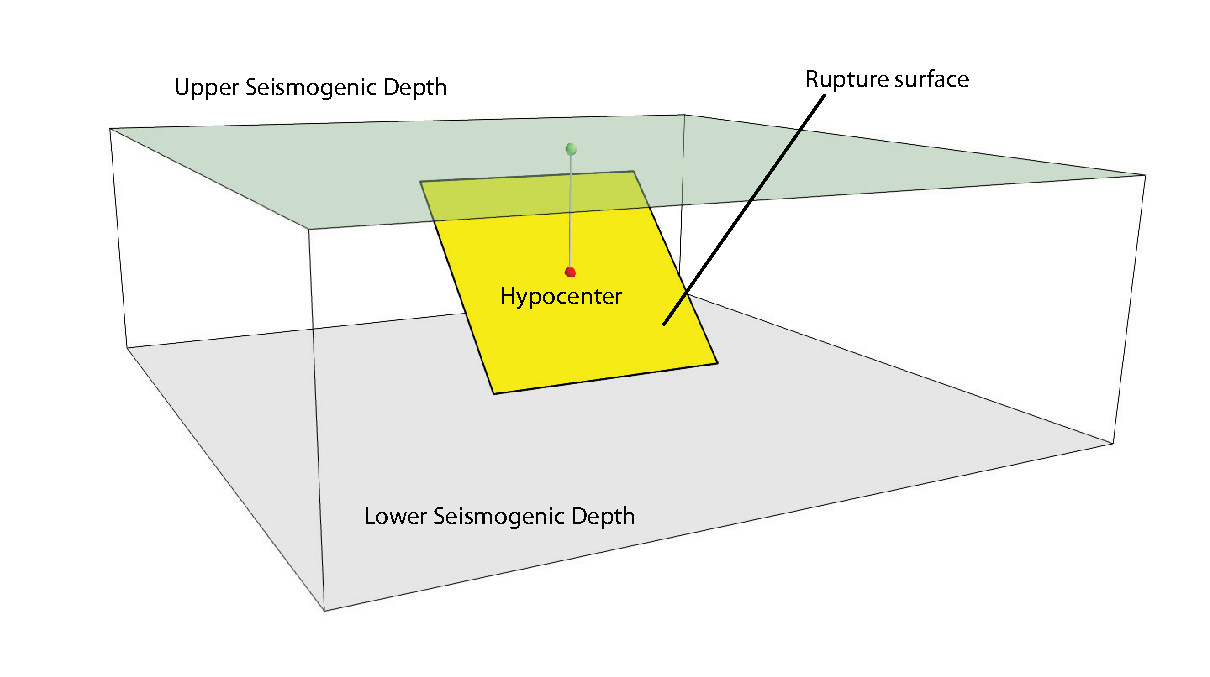
\includegraphics[width=10cm]{figures/hazard/single_rupture.pdf}
	\end{figure}}
}


\newglossaryentry{fragilityfunction}{
	name=fragility function,
	description={the probability of exceeding a set of limit states, given
	an intensity measure level. These functions can be discrete or continuous}
}


\newglossaryentry{fragilitymodel}{
	name=fragility model,
	description={A set of \glspl{vulnerabilityfunction} used to model the
	fragility of all the \glspl{asset} in the \gls{exposuremodel}}
}


\newglossaryentry{frequencymagnitudedistribution}{
	name=frequency-magnitude distribution,
	description={See \gls{mfd}}
}



% ------- G

\newacronym{acr:gem}{GEM}{Global Earthquake Model}
\newacronym{acr:gmf}{GMF}{Ground Motion Field}
\newacronym{acr:gmpe}{GMPE}{Ground Motion Prediction Equation}
\newacronym{acr:gmlt}{GMLT}{Ground Motion Logic Tree (see \gls{groundmotionlogictree}}


\newglossaryentry{gridsource}{
	name=grid source,
	description={A source typology usually adopted to model distributed
	seismicity. It is routinely produced by a seismicity smoothing algorithm (one
	of the most famous algorithm is the one proposed by \citet{frankel1995})}
}


\newglossaryentry{groundmotionfield}{
	name=ground-motion field,
	description={An object describing the geographic distribution around a
	rupture of a ground motion intensity measure}
}


\newglossaryentry{groundmotionfieldcalc}{
	name=ground-motion field calculator,
	description={An \gls{acr:oqe} calculator that given a rupture computes the
	geographic distribution of a ground motion intensity parameter. Currently
	OQ can generate ground motion fields using a \gls{acr:gmpe}}
}


\newglossaryentry{groundmotionlogictree}{
	name=ground-motion logic tree,
	description={A method used to systematically describe the epistemic
	uncertainties related to the ground motion models used in the computation
	of hazard using a specific \gls{pshainputmodel}}
}


\newglossaryentry{groundmotionmodel}{
	name=ground-motion model,
	description={An object that given a rupture with specific properties
	computes the expected ground motion at the given site. In simplest case a
	ground motion model corresponds to a \gls{groundmotionpredictioneq}. In
	case of complex PSHA input models, the produced ground motion models
	contains a set of \glspl{acr:gmpe}, one for each tectonic region considered}
}


\newglossaryentry{groundmotionparameter}{
	name=ground-motion parameter,
	description={A scalar or vector quantity describing a relevant property
	of the shaking such as intensity (e.g. PGA or Spectral Acceleration)
	or duration, equivalent number of cycles  \citep[see for
	example][]{hancock2005})}
}


\newglossaryentry{groundmotionpredictioneq}{
	name=ground-motion prediction equation,
	description={An equation that - given some fundamental parameters
	characterizing  the source, the propagation path and the site (in the
	simplest  case magnitude, distance and V$_\text{S,30}$) - computes the
	value $GM$ of a (scalar) ground motion intensity parameter}
}


\newglossaryentry{groundmotionsystem}{
	name=ground-motion system,
	description={An object containing a list of \gls{groundmotionlogictree}}
}



% ------- I

\newglossaryentry{initialseismicsourceinputmodel}{
	name=initial seismic source input model,
	description={It is the ensable of information needed to fully describe
	the seismic sources composing a seismic source input model. The
	initial seismic source input model is included in the first branching
	level of a seismic source logic tree}
}


\newglossaryentry{insuredlosses}{
	name=insured losses,
	description={Fraction of the ground-up losses that can be covered by the
	insurance industry, according to a certain policy}
}


\newglossaryentry{investigationtime}{
	name=investigation time,
	description={The time interval considered to calculate hazard; usually
	it corresponds to 50 years}
}



% ------- L

\newglossaryentry{limit}{
	name=limit,
	description={A parameter used in the calculation of insured losses that
	establishes the maximum economic amount that can be covered by the insurance
	industry, according to a certain insurance policy}
}


\newglossaryentry{logictree}{
	name=logic tree,
	description={Data structure used to systematically describe uncertainties
	on parameters and models used in a PSHA study}
}


\newglossaryentry{logictreeprocessor}{
	name=logic tree processor,
	description={An OQ calculator that takes the PSHA Input Model and creates
	many realisations of a \gls{seismicsourcemodel} and of a
	\gls{groundmotionmodel}}
}


\newacronym{acr:ltmcs}{LTMCS}{Logic Tree Monte Carlo Sampler}

%------------M

\newglossaryentry{msr}{
	name=magnitude-scaling relationship,
	description={An empirical relationship linking the magnitude with a
	parameter  describing the size of the corresponding rupture (e.g. the
	area  of the rupture or the rupture length)}
}


\newacronym{acr:mfd}{MFD}{Magnitude-Frequency Distribution}
\newglossaryentry{mfd}{
	name=magnitude-frequency distribution,
	description={A distribution describing the frequency of earthquakes with
	a specific magnitude. It can be continuous or discrete. One frequency-
	magnitude distribution frequently adopted in \gls{acr:psha} is the double
	truncated Gutenberg-Richter distribution}
}

%---------------N
\newglossaryentry{nonparametricsource}{
    name=non-parametric source,
    description={A source typology in which the earthquake rupture forecast is
    described explicitly by a set of ruptures and the corresponding
    probabilities of occurrence}
}



% ------- N

\newacronym{acr:nrml}{NRML}{Natural hazards' Risk Markup Language}
\newglossaryentry{nrml}{
	name=Natural hazards' Risk Markup Language,
	description={A markup language similar to XML, which specifies a number
	of standardised schemas to represent various input models used for
	\gls{acr:oqe} calculations and output files generated by \gls{acr:oqe}
	calculations
	}
}



% ------- O

\newacronym{acr:hazlib}{oq-hazardlib}{OpenQuake hazard library}


\newglossaryentry{opensha}{
	name=OpenSHA,
	description={OpenSHA is an open-source, advanced Java-based platform
	for conducting Seismic Hazard Analysis - (see
	\href{http://opensha.org}{OpenSHA website})}
}


\newacronym{acr:oqe}{oq-engine}{OpenQuake-engine}
\newacronym{acr:oqe17}{oq-engine 1.7}{OpenQuake-engine v1.7}
\newacronym{acr:oqe18}{oq-engine 1.8}{OpenQuake-engine v1.8}
\newacronym{acr:oqe19}{oq-engine 1.9}{OpenQuake-engine v1.9}
\newacronym{acr:oqe20}{oq-engine 2.0}{OpenQuake-engine v2.0}
\newacronym{acr:oqe21}{oq-engine 2.1}{OpenQuake-engine v2.1}
\newacronym{acr:oqe22}{oq-engine 2.2}{OpenQuake-engine v2.2}
\newacronym{acr:oqe23}{oq-engine 2.3}{OpenQuake-engine v2.3}
\newacronym{acr:oqe24}{oq-engine 2.4}{OpenQuake-engine v2.4}



% ------- P

\newacronym{acr:pga}{PGA}{Peak Ground Acceleration}
\newacronym{acr:pgv}{PGV}{Peak Ground Velocity}

\newacronym[description={\glslink{psha}{Probabilistic Seismic Hazard
	Analysis}}]{acr:psha}{PSHA}{Probabilistic Seismic Hazard Analysis}


\newglossaryentry{pointsource}{
	name=point source,
	description={The elemental source typology used in the \glsdesc{acr:oqe} to
	model distributed seismicity}
}


\newglossaryentry{pshainputmodel}{
	name=PSHA input model,
	description={An object containing the information necessary to describe
	the seismic source and the ground motion models - plus the related
	epistemic uncertainties}
}


\newglossaryentry{psha}{
	name=probabilistic seismic hazard analysis,
	description={A methodology to compute seismic hazard by taking into
	account the potential contributions coming from all the sources of
	engineering importance for a specified site}
}



% ------- R

\newacronym{acr:risklib}{oq-risklib}{OpenQuake risk library}


\newacronym{acr:rrup}{$\text{r}_{\text{rup}}$}{closest distance between the
	site and rupture}


\newglossaryentry{rupture}{
	name=earthquake rupture,
	description={A 3D surface - representing a portion or the entire fault
	surface - over which a slip event (i.e. an earthquake) occurs}
}


\newglossaryentry{rupturemodel}{
	name=rupture model,
	description={An object containing the information necessary to describe
	a \gls{rupture}, such as magnitude, hypocenter location, strike, dip, 
	rake, and seismogenic depths}
}


\newglossaryentry{ruptureaspectratio}{
	name=rupture aspect ratio,
	description={The ratio between the lenght and the width of an
	earthquake rupture}
}


\newglossaryentry{rake}{
	name=rake,
	description={The rake is the direction in which a hanging wall block moves
	during a rupture, measured relative to fault strike on the plane of the
	fault}
}



% ------- S

\newacronym{acr:ssha}{SSHA}{Scenario Based Seismic Hazard Analysis}


\newglossaryentry{scenariohazard}{
	name=scenario based seismic hazard analysis,
	plural=scenario based seismic hazard analyses,
	description={An analyis of seismic hazard based on the selection of
	one or a few ruptures and the computation of the expected ground
	motion at a set of sites using a \gls{gmpe} accounting ground motion
	variability}
}


\newglossaryentry{seismicityhistory}{
	name=seismicity history,
	plural=seismicity histories,
	description={An object containing a set ruptures representative of the
	possible seismicity generated by the sources in a
	\gls{seismicsourcemodel} during the investigation time $t$}
}


\newglossaryentry{seismicityrate}{
	name=seismicity rate,
	description={Number of events per unit of time (if not better
	specified, the definition of a seismicity rate generally presumes a time
	independent}
}


\newglossaryentry{seismicsourcedata}{
	name=seismic source data,
	description={An object containing the information necessary to
	completely describe a \gls{acr:psha} seismic source i.e. seismic source
	type, position, geometry and seismicity occurrence model}
}


\newglossaryentry{seismicsourcelogictree}{
	name=seismic source logic tree,
	description={Logic tree structure defined to describe in structured and
	systematic way the epistemic uncertainties characterizing the seismic
	source model. The first branching level in the logic tree by definition
	contains one or several alternative \gls{initialseismicsourceinputmodel}}
}


\newacronym{acr:ssim}{SSIM}{Seismic Source Input Model}


\newglossaryentry{seismicsourceinputmodel}{
	name=seismic source input model,
	description={An object containing a list of \gls{seismicsourcedata}. In
	the \glsdesc{acr:oqe} a seismic source model doesn't contain epistemic
	uncertainty}
}


\newglossaryentry{seismicsource}{
	name=seismic source,
	description={An object that can generate}}


\newacronym{acr:ssm}{SSM}{Seismic Source Model}
\newglossaryentry{seismicsourcemodel}{
	name=seismic source model,
	description={An object containing a list of \glspl{seismicsource}
	objects}
}


\newacronym{acr:scec}{SCEC}{Southern California Earthquake Center}


\newglossaryentry{seismicsourcesystem}{
	name=seismic source system,
	description={An object containing a list of
	\glspl{initialseismicsourceinputmodel} and the
	\gls{seismicsourcelogictree}}
}


\newglossaryentry{simplefaultsource}{
	name=simple fault source,
	description={A source typology usually adopted to model shallow
	structures with an uncomplicated geometry}
}


\newacronym{acr:ses}{SES}{Stochastic Event Set}
\newglossaryentry{stochasticeventset}{
	name=stochastic event set,
	description={An object containing one or many \glspl{seismicityhistory}}
}


\newglossaryentry{strike}{
	name=strike,
	description={The strike direction correspond to the angle between the
	north and the direction you take so that when you walk along the
	\gls{faulttrace} the fault dips on your right}
}


\newacronym{acr:sa}{S$_a$}{Spectral Acceleration}



% ------- T

\newglossaryentry{taxonomy}{
	name=taxonomy,
	plural=taxonomies,
	description={Scheme used to classify the \glspl{asset}. For buildings, a
	classification scheme has been proposed by \gls{acr:gem} which considers a
	number of attributes including lateral load resisting system and its
	material, height, year of construction. The taxonomy is currently used to
	link the \glspl{asset} in the \gls{exposuremodel} to the relevant
	\gls{vulnerabilityfunction} or \gls{fragilityfunction}}
}


\newglossaryentry{tectonicregion}{
	name=tectonic region,
	description={A area on the topographic surface that can be considered
	homogeneous in terms of tectonic properties such as the prevalent
	seismogenic properties and/or the seismic wave propagation properties}
}


\newglossaryentry{temporaloccurrencemodel}{
	name=temporal occurrence model,
	description={Usually a probabilistic model giving the probability of
	occurrence of an event in a specified \gls{investigationtime}}
}



% ------- U

\newacronym{acr:usgs}{USGS}{United States Geological Survey}



% ------- V

\newglossaryentry{vulnerabilityfunction}{
	name=vulnerability function,
	description={A function that describes the probability distribution of
	loss ratio, conditioned on an intensity measure level. Currently only
	discrete vulnerability functions are supported}
}


\newglossaryentry{vulnerabilitymodel}{
	name=vulnerability model,
	description={A set of \glspl{vulnerabilityfunction} used to model the
	physical vulnerability of all the \glspl{asset} in the \gls{exposuremodel}}
}


\newglossaryentry{acr:vs30}{
	name=V$_{S,30}$,
	description={Average shear wave velocity of the materials in the uppermost
	30m of the soil column}
}
 % ---------------------------------------- Load glossary -

\begin{document}

%-------------------------------------------------------------------------------
%  COVER PAGE
%-------------------------------------------------------------------------------

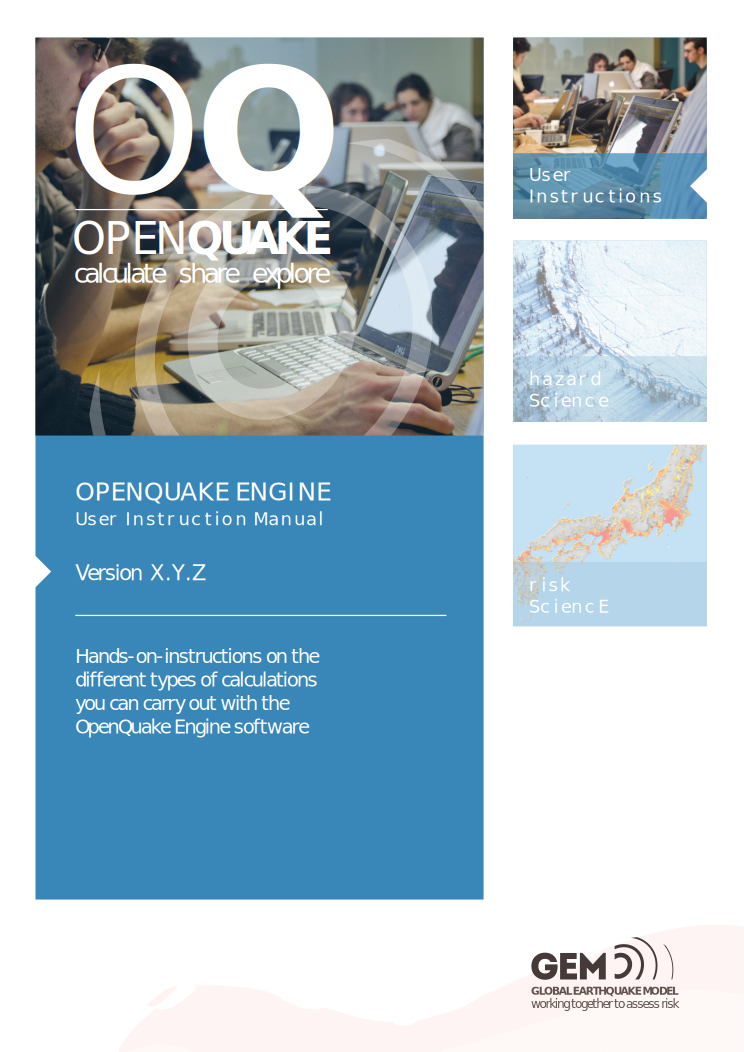
\includepdf[pages=-]{figures/oq_manual_cover.pdf}

%-------------------------------------------------------------------------------
%  TITLE PAGE
%-------------------------------------------------------------------------------

\begingroup
\thispagestyle{empty}
\begin{center}
\par\normalfont\fontsize{15}{15}\sffamily\selectfont
\textcolor{oqblue}{OpenQuake: calculate, share, explore}
\vspace*{9cm}
\par\bfseries\fontsize{35}{35}\sffamily\selectfont
\textcolor{gembrown}{The OpenQuake-engine\\User Instruction Manual}\par
\vspace*{9cm}
\par\normalfont\fontsize{15}{15}\sffamily\selectfont
\href{http://globalquakemodel.org/openquake/}{\textcolor{oqblue}{globalquakemodel.org/openquake}}
\end{center}
\endgroup

%-------------------------------------------------------------------------------
%  COPYRIGHT PAGE
%-------------------------------------------------------------------------------

\newpage
~\vfill
\thispagestyle{empty}

\noindent
   \textbf{Authors} \\
   Marco Pagani$^1$, Vitor Silva$^1$,
   Anirudh Rao$^1$, Michele Simionato$^1$,
   Robin Gee$^1$, Kendra Johnson$^1$\hfill \\
   \hfill \\
   \textbf{Authors on previous versions} \\
   Helen Crowley$^2$, Damiano Monelli, Graeme Weatherill$^3$\hfill \\
   \hfill \\
   \small
   \begin{tabular}{p{4cm}p{4cm}p{4cm}}
   $^1$ GEM Foundation \hfill \newline
   via Ferrata, 1 \hfill \newline
   20133 Pavia \hfill \newline
   Italy \hfill \newline
   &
   $^2$ EUCENTRE \hfill \newline
   via Ferrata, 1 \hfill \newline
   20133 Pavia \hfill \newline
   Italy \hfill \newline
   &
   $^3$ GFZ \hfill \newline
   Helmholtzstraße 6/7 \hfill \newline
   14467 Potsdam \hfill \newline
   Germany \hfill \newline
   \end{tabular} \hfill \newline
   %
   Email address for all current authors:\hfill\\
   $<$firstname.lastname$>$@globalquakemodel.org\hfill\\
   \normalsize

\noindent
   {\textbf{Citation}} \hfill \\
   Please cite this document as: \hfill \\
   GEM (#PUBYEAR#). The OpenQuake-engine User Manual.
   \textit{Global Earthquake Model (GEM) OpenQuake Manual for Engine version X.Y.Z.\\
   doi: 10.13117/GEM.OPENQUAKE.MAN.ENGINE.X.Y.Z, \pageref{LastPage} pages.} \hfill \\
\noindent \hfill\\
\noindent
   {\bf{Disclaimer}} \hfill \\
   The OpenQuake-engine User Manual is distributed in the hope that it will be
   useful, but without any warranty: without even the implied warranty of
   merchantability or fitness for a particular purpose. While every precaution
   has been taken in the preparation of this document, in no event shall the
   authors of the Manual and the GEM Foundation be liable to any party for
   direct, indirect, special, incidental, or consequential damages, including
   lost profits, arising out of the use of information contained in this
   document or from the use of programs and source code that may accompany it,
   even if the authors and GEM Foundation have been advised of the possibility
   of such damage. The Manual provided hereunder is on as ``as is'' basis, and
   the  authors and GEM Foundation have no obligations to provide maintenance,
   support, updates, enhancements, or modifications. \hfill \\
\noindent \hfill\\
\noindent
   {\bf{License}} \hfill \\
   This Manual is distributed under the Creative Commons License  Attribution-
   NonCommercial-ShareAlike 4.0 International
   (\href{http://creativecommons.org/licenses/by-nc-sa/4.0/} {CC BY-NC-SA
   4.0}). You can download this Manual and share it with others as long as you
   provide proper credit, but you cannot change it in any way or use it
   commercially.\hfill \\

\noindent \copyright\ \textsc{2013--#PUBYEAR# GEM Foundation}\\
\noindent \textit{#PUBMONTH# #PUBYEAR#} % Printing/edition date

%-------------------------------------------------------------------------------
%  TABLE OF CONTENTS
%-------------------------------------------------------------------------------

\chapterimage{figures/chapter_head.pdf} % Table of contents heading image
\pagestyle{empty} % No headers
\tableofcontents % Print the table of contents itself
\cleardoublepage % Forces the first chapter to start on the right
\pagestyle{fancy} % Print headers again

%-------------------------------------------------------------------------------
%  FOREWORD
%-------------------------------------------------------------------------------
\chapterimage{figures/chapter_head.pdf} % Chapter heading image
\chapter*{Preface}
\addcontentsline{toc}{chapter}{Preface}
The goal of this manual is to provide a comprehensive and transparent
description of the features of the OpenQuake Engine. This manual is
designed to be readable by someone with basic understanding of Probabilistic
Seismic Hazard and Risk Analysis, but no previous knowledge of the
\glsdesc{acr:oqe} is assumed.

The \glsdesc{acr:oqe} is an effort promoted and actively developed by the
\glsdesc{acr:gem}, a public-private partnership initiated by the
Global Science Forum of the Organisation for Economic Co-operation and Development
(OECD)\footnote{A short description of the process promoted by OECD is available here:\\\href{http://www.oecd.org/science/sci-tech/theglobalearthquakemodelgem.htm}{http://www.oecd.org/science/sci-tech/theglobalearthquakemodelgem.htm}}.

The \glsdesc{acr:oqe} is the result of an effort carried out jointly by the
Information Technology and Scientific teams working at the \gls{acr:gem} Secretariat.
It is freely distributed under an Affero GPL license
(\href{http://www.gnu.org/licenses/agpl-3.0.html}{http://www.gnu.org/licenses/agpl-3.0.html}).


%-------------------------------------------------------------------------------
%  THE MANUAL
%-------------------------------------------------------------------------------

% ------------------------------------------------------- Part I: Introduction -
\part{Introduction}
\label{part:introduction}
\chapterimage{figures/chapter_head.pdf} % Chapter heading image
\chapter{OpenQuake-engine Background}
   \label{chap:intro}
	\section{Overview}

OpenQuake-engine is the seismic hazard and risk calculation software developed by
the \glsdesc{acr:gem}. By following current standards in software
developments like test-driven development and continuous integration, the
\glsdesc{acr:oqe} aims at becoming an open, and community-driven tool for
seismic hazard and risk analysis.

The source code of the \glsdesc{acr:oqe} is available on a public web-based
repository at the following address:
\href{http://github.com/gem/oq-engine}{http://github.com/gem/oq-engine}.

The \glsdesc{acr:oqe} is available for the Linux, macOS, and Windows
platforms. It can be installed in several different ways. The following page
provides a handy guide for users to choose the most appropriate installation
method depending on their intended use cases:

\href{https://github.com/gem/oq-engine/blob/master/doc/installing/README.md}{https://github.com/gem/oq-engine/blob/master/doc/installing/README.md}.

This user manual is for the command line interface for the \glsdesc{acr:oqe}.


\section{Supplementary resources}

Guidance instructions for using the \glsdesc{acr:oqe} WebUI are available 
at \href{https://github.com/gem/oq-engine/blob/master/doc/running/server.md}{https://github.com/gem/oq-engine/blob/master/doc/running/server.md}.

A user manual for the QGIS plugin for the \glsdesc{acr:oqe} is available at 
\href{https://docs.openquake.org/oq-irmt-qgis/latest/}{https://docs.openquake.org/oq-irmt-qgis/latest/}. 
In particular, instructions for using the plugin as an interface for running \glsdesc{acr:oqe}
calculations are listed in Chapter 14, and methods for using the plugin for visualization 
of hazard and risk outputs are listed in Chapter 15.

A manual intended for more advanced users of the \glsdesc{acr:oqe} is available
at \href{https://docs.openquake.org/oq-engine/advanced/OpenQuakeforAdvancedUsers.pdf}{https://docs.openquake.org/oq-engine/advanced/OpenQuakeforAdvancedUsers.pdf}.

Interested users are also encouraged to peruse the \href{https://storage.globalquakemodel.org/media/cms_page_media/432/oqhbt_BkpnqP8.pdf}{OpenQuake Hazard Science} and \href{https://storage.globalquakemodel.org/media/cms_page_media/432/oq-risk-manual-1_0.pdf}{OpenQuake Risk Science} books, which 
provide explanations of the scientific methodologies adopted in the implementation
of the earthquake hazard and risk libraries of the \glsdesc{acr:oqe}.

Subscribe to the OpenQuake users mailing list to keep abreast of the latest 
announcements from the OpenQuake development team, to ask and answer questions
related to the \glsdesc{acr:oqe} and participate in the ongoing discussions: 
\href{https://groups.google.com/g/openquake-users}{https://groups.google.com/g/openquake-users}



\section{Launching a calculation}

An \gls{acr:oqe} analysis is launched from the command line of a terminal.

A schematic list of the options that can be used for the execution of the
\gls{acr:oqe} can be obtained with the following command:

\begin{minted}[fontsize=\footnotesize,frame=single,bgcolor=lightgray]{shell-session}
user@ubuntu:~\$ oq engine --help
\end{minted}

The result is the following:
\inputminted[firstline=1,fontsize=\footnotesize,frame=single]{shell-session}{oqum/help.txt}


% ----------------------------------------------------- Part II: Hazard Module -
\thispagestyle{empty}
\part{Hazard}

\chapterimage{figures/chapter_head.pdf} % Chapter heading image
\chapter{Introduction to the Hazard Module}
   \label{chap:hazintro}
	\index{OpenQuake-engine!Risk}

The seismic risk results are calculated using the \gls{acr:risklib}, 
an open-source suite of tools for seismic risk assessment and
loss estimation. This library is written in the Python programming language
and available in the form of a ``developers'' release at the following location:
\href{https://github.com/gem/oq-engine/tree/master/openquake/risklib}{https://github.com/gem/oq-engine/tree/master/openquake/risklib}.

The risk component of the \glsdesc{acr:oqe} can compute both scenario-based and
probabilistic seismic damage and risk using various approaches. The following
types of analysis are currently supported:

\begin{itemize}

    \item \textit{\textbf{Scenario Damage Assessment}}, for the
	calculation of damage distribution statistics for a portfolio of buildings
	from a single earthquake rupture scenario taking into account aleatory and
	epistemic ground-motion variability.

    \item \textit{\textbf{Scenario Risk Assessment}}, for the calculation of
	individual asset and portfolio loss statistics due to a single earthquake
	rupture scenario taking into account aleatory and epistemic ground-motion
	variability. Correlation in the vulnerability of different assets of the
	same typology can also be taken into consideration.

	\item \textit{\textbf{Classical Probabilistic Seismic Damage Analysis}}, for 
	the calculation of damage state probabilities over a specified time period,  
	and probabilistic collapse maps, starting from the hazard curves 
	computed following the classical integration procedure (\cite{cornell1968}, 
	\citet{mcguire1976}) as formulated by \cite{field2003}.

    \item \textit{\textbf{Classical Probabilistic Seismic Risk Analysis}}, for the
	calculation of loss curves and loss maps, starting from the hazard curves 
	computed following the classical integration procedure (\cite{cornell1968}, 
	\citet{mcguire1976}) as formulated by \cite{field2003}.

	\item \textit{\textbf{Stochastic Event Based Probabilistic Seismic Damage Analysis}}, 
	for the calculation of event damage tables starting from stochastic event sets.
	Other results such as damage-state-exceedance curves, probabilistic damage maps, 
	and average annual damages or collapses can be obtained by 
	post-processing the event damage tables.

	\item \textit{\textbf{Stochastic Event Based Probabilistic Seismic Risk Analysis}}, 
	for the calculation of event loss tables starting from stochastic event sets.
	Other results such as loss-exceedance curves, probabilistic loss maps, 
	and average annual losses can be obtained by 
	post-processing the event loss tables.

    \item \textit{\textbf{Retrofit Benefit-Cost Ratio Analysis}}, which is
	useful in estimating the net-present value of the potential benefits of
	performing retrofitting for a portfolio of assets (in terms of decreased
	losses in seismic events), measured relative to the upfront cost of
	retrofitting.

\end{itemize}

Each calculation workflow has a modular structure, so that intermediate
results can be saved and analyzed. Moreover, each calculator can be
extended independently of the others so that additional calculation options
and methodologies can be easily introduced, without affecting the overall
calculation workflow. Each workflow is described in more detail in the
following sections.

\section{Scenario Damage Assessment}
\index{OpenQuake-engine!Risk calculation workflows!Scenario Damage Assessment}
\label{sec:workflow_scenario_damage}
The scenario damage calculator computes damage distribution statistics for all
\glspl{asset} in a given \gls{exposuremodel} for a single specified
\gls{rupture}. Damage distribution statistics include the mean and standard
deviation of damage fractions for different damage states. This calculator
requires the definition of a finite \gls{rupturemodel}, an \gls{exposuremodel}
and a \gls{fragilitymodel}; the main results are the damage distribution
statistics per \gls{asset}, aggregated damage distribution statistics per
taxonomy, aggregated damage distribution statistics for the region, and
collapse maps, which contain the spatial distribution of the number or area of
collapsed buildings throughout the region of interest.

The \gls{rupture} characteristics---i.e. the magnitude, hypocenter and fault
geometry---are modelled as deterministic in the scenario calculators. Multiple
simulations of different possible \glspl{acr:gmf} due to the single
\gls{rupture} are generated, taking into consideration both the inter-event
variability of ground motions, and the intra-event residuals obtained from a
spatial correlation model for ground motion residuals. The use of logic trees
allows for the consideration of uncertainty in the choice of a ground motion
model for the given tectonic region.

As an alternative to computing the \glspl{acr:gmf} with \glsdesc{acr:oqe},
users can also provide their own sets of \glspl{acr:gmf} as input to the
scenario damage calculator.

\textbf{Note}: The damage simulation algorithm for the scenario damage 
calculator has changed starting from \glsdesc{acr:oqe39} to use a full
Monte Carlo simulation of damage states.

For each \gls{acr:gmf}, a damage state is simulated for each building for every
\gls{asset} in the \gls{exposuremodel} using the provided \gls{fragilitymodel},
and finally the mean damage distribution across all realizations is calculated.
The calculator also provides aggregated damage distribution statistics for the
portfolio, such as mean damage fractions for each taxonomy in the 
\gls{exposuremodel}, and the mean damage for the entire region of study.

The required input files required for running a scenario damage calculation
and the resulting output files are depicted in Figure~\ref{fig:io-structure-scenario-damage}.

\begin{figure}[ht]
\centering
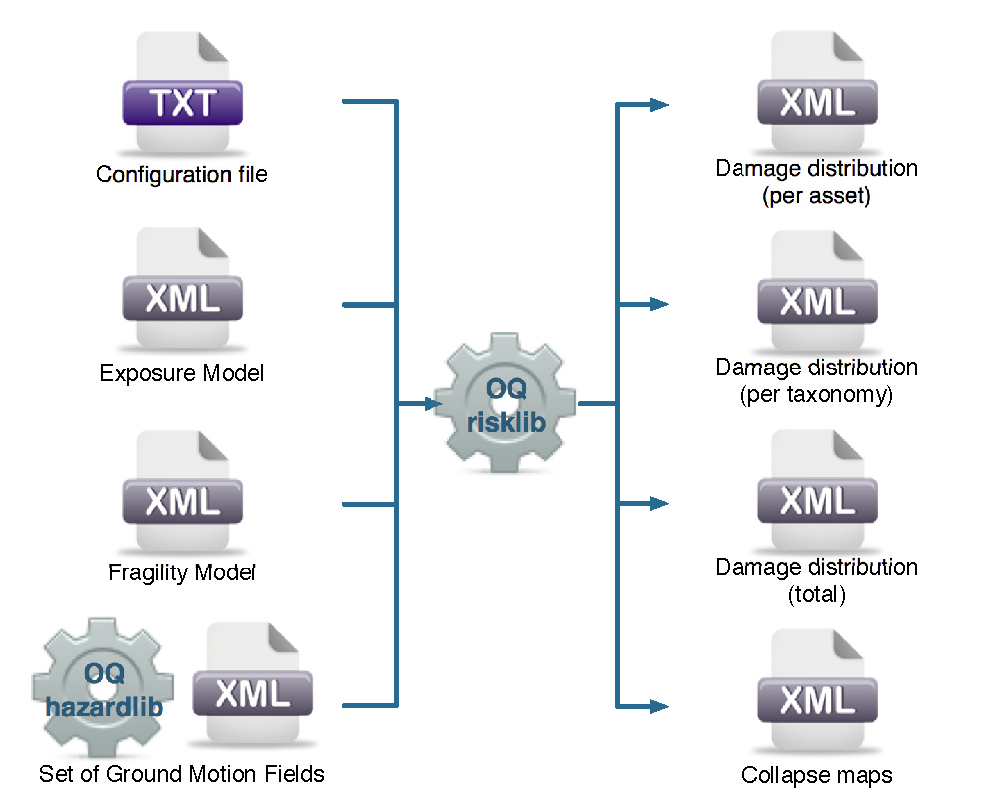
\includegraphics[width=9cm,height=7cm]{figures/risk/io-structure-scenario-damage.pdf}
\caption{Scenario Damage Calculator input/output structure.}
\label{fig:io-structure-scenario-damage}
\end{figure}

\gls{consequencemodel} files can also be
provided as inputs for a scenario damage calculation in addition to
\glspl{fragilitymodel} files, in order to estimate consequences based on the
calculated damage distribution. The user may provide one
\gls{consequencemodel} file corresponding to each loss type (amongst
structural, nonstructural, contents, and business interruption) for which a
\gls{fragilitymodel} file is provided. Whereas providing a
\gls{fragilitymodel} file for at least one loss type is mandatory for running
a Scenario Damage calculation, providing corresponding \gls{consequencemodel}
files is optional.


\section{Scenario Risk Assessment}
\index{OpenQuake-engine!Risk calculation workflows!Scenario Risk Assessment}
\label{sec:workflow_scenario_risk}
The scenario risk calculator computes loss statistics for all \glspl{asset} in
a given \gls{exposuremodel} for a single specified \gls{rupture}.
Loss statistics include the mean and standard deviation of ground-up losses
for each loss type considered in the analysis. Loss
statistics can currently be computed for five different loss types using this
calculator: structural losses, nonstructural losses, contents losses, downtime
losses, and occupant fatalities. This calculator requires the definition of a
finite \gls{rupturemodel}, an \gls{exposuremodel} and a
\gls{vulnerabilitymodel} for each loss type considered; the main results are
the loss statistics per \gls{asset} and mean loss maps.

The \gls{rupture} characteristics---i.e. the magnitude, hypocenter and fault
geometry---are modelled as deterministic in the scenario calculators. Multiple
simulations of different possible \glspl{acr:gmf} due to the single
\gls{rupture} are generated, taking into consideration both the inter-event
variability of ground motions, and the intra-event residuals obtained from a
spatial correlation model for ground motion residuals. The use of logic trees
allows for the consideration of uncertainty in the choice of a ground motion
model for the given tectonic region.

As an alternative to computing the \glspl{acr:gmf} with OpenQuake, users can
also provide their own sets of \glspl{acr:gmf} as input to the scenario risk
calculator.

For each \gls{acr:gmf} simulation, a loss ratio is sampled for every asset in
the \gls{exposuremodel} using the provided probabilistic
\gls{vulnerabilitymodel} taking into consideration the correlation model for
vulnerability of different \glspl{asset} of a given taxonomy. Finally loss
statistics, i.e., the mean loss and standard deviation of loss for
ground-up losses across all simulations, are calculated
for each \gls{asset}. Mean loss maps are also generated by this calculator,
describing the mean ground-up losses caused by the
scenario event for the different assets in the \gls{exposuremodel}.

The required input files required for running a scenario risk calculation and
the resulting output files are depicted in Figure~\ref{fig:io-structure-scenario-risk}.

\begin{figure}[ht]
\centering
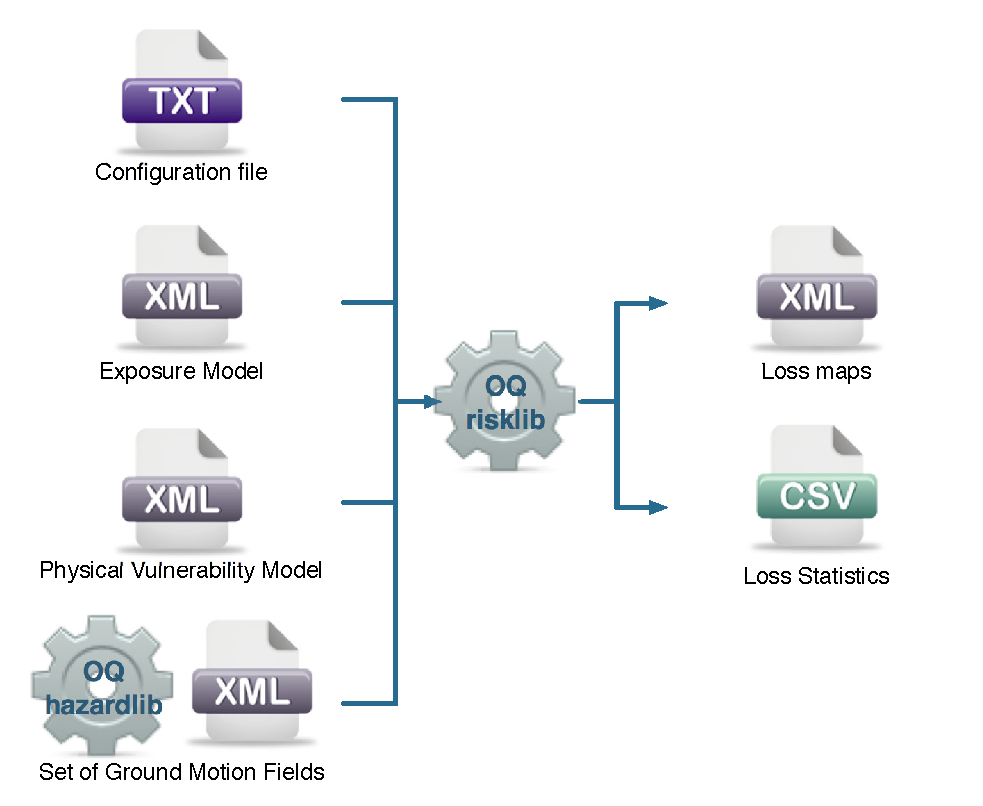
\includegraphics[width=9cm,height=7cm]{figures/risk/io-structure-scenario-risk.pdf}
\caption{Scenario Risk Calculator input/output structure.}
\label{fig:io-structure-scenario-risk}
\end{figure}


\section{Classical Probabilistic Seismic Damage Analysis}
\index{OpenQuake-engine!Risk calculation workflows!Classical Probabilistic Seismic Damage Analysis}
\label{sec:workflow_classical_damage}
\input{oqum/risk/00_workflow_classical_damage}

\section{Classical Probabilistic Seismic Risk Analysis}
\index{OpenQuake-engine!Risk calculation workflows!Classical Probabilistic Seismic Risk Analysis}
\label{sec:workflow_classical_risk}
\input{oqum/risk/00_workflow_classical_risk}

\section{Stochastic Event Based Probabilistic Seismic Damage Analysis}
\index{OpenQuake-engine!Risk calculation workflows!Event-Based Probabilistic Seismic Damage Analysis}
\label{sec:workflow_event_based_damage}
This calculator employs an event-based Monte Carlo simulation approach to
probabilistic damage assessment in order to estimate the damage distribution for
individual \glspl{asset} and aggregated damage distribution for a spatially
distributed portfolio of \glspl{asset} within a specified time period. The
calculator requires the definition of an \gls{exposuremodel}, a
\gls{fragilitymodel} for each loss type of interest with
\glspl{fragilityfunction} for each damage state for every typology represented 
in the \gls{exposuremodel}, and a \glsdesc{acr:ses} representative of the 
seismicity of the region over the specified time period. Damage state curves 
and damage maps corresponding to specified return periods can also be 
obtained using this calculator.

As an alternative to computing the \glspl{acr:gmf} with \glsdesc{acr:oqe},
users can also provide their own sets of \glspl{acr:gmf} as input to the
event-based damage calculator.

The main results of this calculator are the event damage tables; these 
tables describe the total number of buildings in each damage state for the
portfolio of \glspl{asset} for each seismic event in the \gls{acr:ses}.

Asset-level event damage tables are generated by the calculator, but are
not exportable in csv format due to the large file sizes that may be
involved. Interested users can access the asset-level event damage tables
within the datastore for the completed calculation.

% Uncomment after the addition of damage curves output
% Damage exceedance curves for each \gls{asset}, which describe 
% the probability of exceedance of different damage levels over the 
% specified time period, and damage maps for the region, which describe the 
% level of damage (for a given damage state) that has a given
% probability of exceedance over the specified time period. Aggregate damage
% exceedance curves can also be produced using this calculator; these
% describe the probability of exceedance of different damage levels for all
% \glspl{asset} in the portfolio.

This calculator relies on the probabilistic event-based hazard calculator,
which simulates the seismicity of the chosen time period $T$ by producing a
\gls{acr:ses}. For each \gls{rupture} generated by a \gls{seismicsource}, the
number of occurrences in the given time span $T$ is simulated by sampling the
corresponding probability distribution as given by $P_{rup}(k | T)$. A
\gls{acr:ses} is therefore a \textit{sample} of the full population of
\glspl{rupture} as defined by a \glsdesc{acr:ssm}. Each \gls{rupture} is
present zero, one or more times, depending on its probability. Symbolically,
we can define a \gls{acr:ses} as:
\begin{align}
SES(T) = \left\{k \times rup,\;k\sim P_{rup}(k | T)\;\;\forall\;rup\;in\;Src\;\forall\;Src\;in\;SSM\right\}
\end{align}
where $k$, the number of occurrences, is a random sample of $P_{rup}(k | T)$,
and $k \times rup$ means that \gls{rupture} $rup$ is repeated $k$ times in the
\gls{acr:ses}.

For each \gls{rupture} or event in the \glspl{acr:ses}, a spatially correlated
\gls{acr:gmf} realisation is generated, taking into consideration both the
inter-event variability of ground motions, and the intra-event residuals
obtained from a spatial correlation model for ground motion residuals (if one 
is specified in the job file). The use of logic trees allows for the 
consideration of uncertainty in the choice of a \glsdesc{acr:ssm}, and in the 
choice of \glspl{groundmotionmodel} for the different tectonic regions.

For each \gls{acr:gmf} realization, a damage state is siumulated for each
building of every \gls{asset} in the \gls{exposuremodel} using the provided
\gls{fragilitymodel}. The asset-level event damage table is saved to the datastore.
Time-averaged damage distributions at the asset-level can be obtained from
the event damage table. Finally damage state exceedance curves can be computed.

The required input files required for running a probabilistic stochastic
event-based damage calculation and the resulting output files are depicted in
Figure~\ref{fig:io-structure-event-based-damage}

\begin{figure}[ht]
\centering
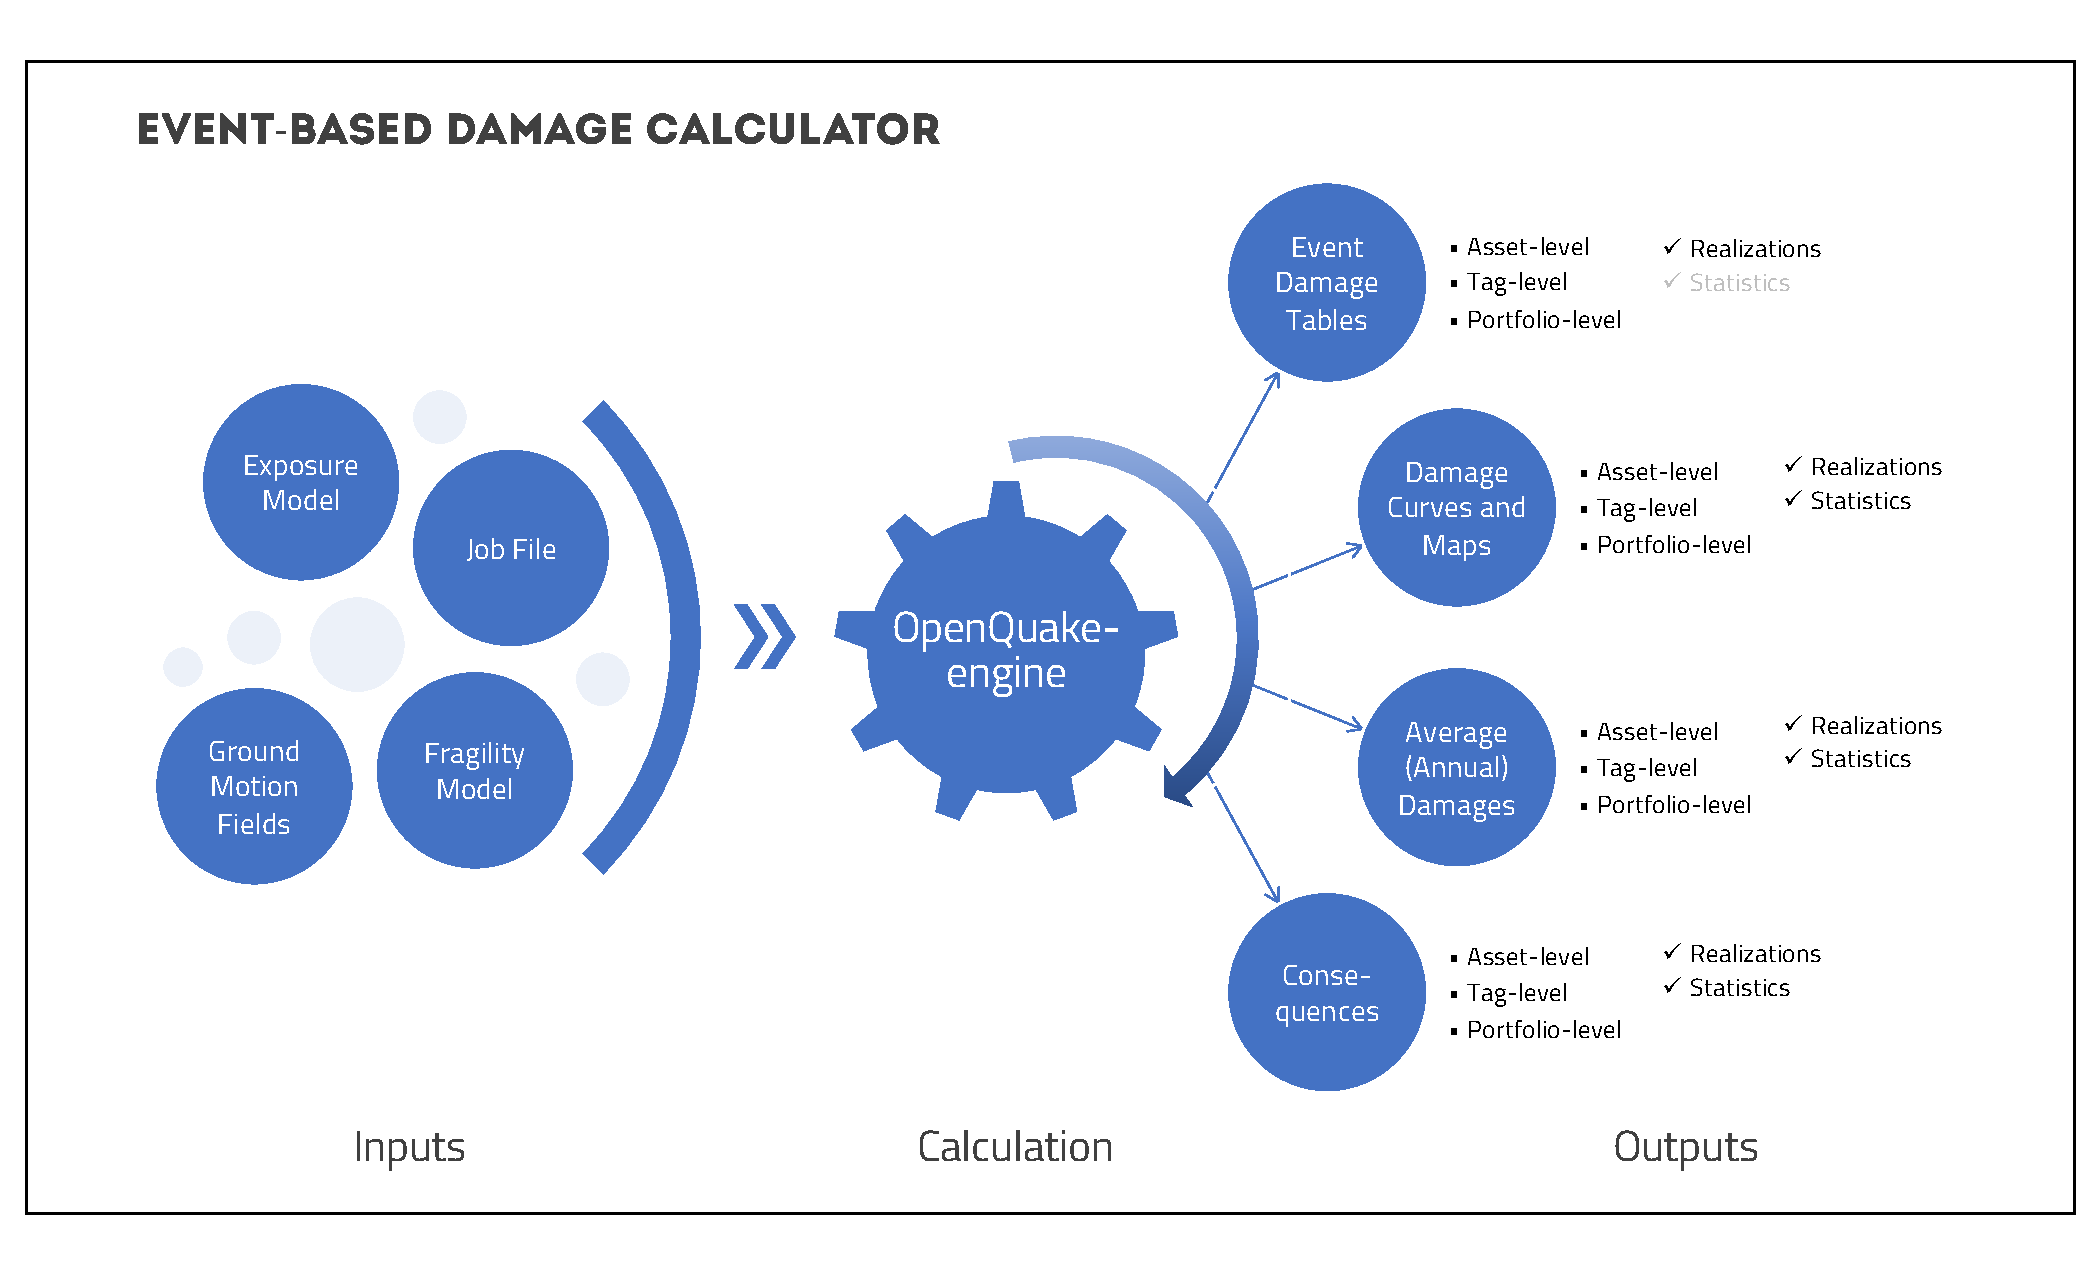
\includegraphics[width=12cm]{figures/risk/io-structure-event-based-damage.pdf}
\caption{Probabilistic Event-based Damage Calculator input/output structure.}
\label{fig:io-structure-event-based-damage}
\end{figure}

Similar to the scenario damage calculator, \gls{consequencemodel} files can also be
provided as inputs for an event-based damage calculation in addition to
\glspl{fragilitymodel} files, in order to estimate consequences based on the
calculated damage distribution. The user may provide one
\gls{consequencemodel} file corresponding to each loss type (amongst
structural, nonstructural, contents, and business interruption) for which a
\gls{fragilitymodel} file is provided. Whereas providing a
\gls{fragilitymodel} file for at least one loss type is mandatory for running
an Event-Based Damage calculation, providing corresponding \gls{consequencemodel}
files is optional.


\section{Stochastic Event Based Probabilistic Seismic Risk Analysis}
\index{OpenQuake-engine!Risk calculation workflows!Event-Based Probabilistic Seismic Risk Analysis}
\label{sec:workflow_event_based_risk}
This calculator employs an event-based Monte Carlo simulation approach to
probabilistic risk assessment in order to estimate the loss distribution for
individual \glspl{asset} and aggregated loss distribution for a spatially
distributed portfolio of \glspl{asset} within a specified time period. The
calculator requires the definition of an \gls{exposuremodel}, a
\gls{vulnerabilitymodel} for each loss type of interest with
\glspl{vulnerabilityfunction} for each taxonomy represented in the
\gls{exposuremodel}, and a \glsdesc{acr:ses} (also known as a
\textit{synthetic catalog}) representative of the seismicity of the region
over the specified time period. Loss curves and loss maps can currently be
calculated for five different loss types using this calculator: structural
losses, nonstructural losses, contents losses, downtime losses, and occupant
fatalities.

As an alternative to computing the \glspl{acr:gmf} with \glsdesc{acr:oqe},
users can also provide their own sets of \glspl{acr:gmf} as input to the
event-based risk calculator, starting from \gls{acr:oqe28}.

The main results of this calculator are loss
exceedance curves for each \gls{asset}, which describe the probability of
exceedance of different loss levels over the specified time period, and loss
maps for the region, which describe the loss values that have a given
probability of exceedance over the specified time period. Aggregate loss
exceedance curves can also be produced using this calculator; these
describe the probability of exceedance of different loss levels for all
\glspl{asset} in the portfolio. Finally, event loss tables can be produced
using this calculator; these tables describe the total loss across the
portfolio for each seismic event in the \gls{acr:ses}.

This calculator relies on the probabilistic event-based hazard calculator,
which simulates the seismicity of the chosen time period $T$ by producing a
\gls{acr:ses}. For each \gls{rupture} generated by a \gls{seismicsource}, the
number of occurrences in the given time span $T$ is simulated by sampling the
corresponding probability distribution as given by $P_{rup}(k | T)$. A
\gls{acr:ses} is therefore a \textit{sample} of the full population of
\glspl{rupture} as defined by a \glsdesc{acr:ssm}. Each \gls{rupture} is
present zero, one or more times, depending on its probability. Symbolically,
we can define a \gls{acr:ses} as:
\begin{align}
SES(T) = \left\{k \times rup,\;k\sim P_{rup}(k | T)\;\;\forall\;rup\;in\;Src\;\forall\;Src\;in\;SSM\right\}
\end{align}
where $k$, the number of occurrences, is a random sample of $P_{rup}(k | T)$,
and $k \times rup$ means that \gls{rupture} $rup$ is repeated $k$ times in the
\gls{acr:ses}.

For each \gls{rupture} or event in the \glspl{acr:ses}, a spatially correlated
\gls{acr:gmf} realisation is generated, taking into consideration both the
inter-event variability of ground motions, and the intra-event residuals
obtained from a spatial correlation model for ground motion residuals (if one 
is specified in the job file). The use of logic trees allows for the 
consideration of uncertainty in the choice of a \glsdesc{acr:ssm}, and in the 
choice of \glspl{groundmotionmodel} for the different tectonic regions.

For each \gls{acr:gmf} realization, a loss ratio is sampled for every
\gls{asset} in the \gls{exposuremodel} using the provided probabilistic
\gls{vulnerabilitymodel}, taking into consideration the correlation model for
vulnerability of different \glspl{asset} of a given taxonomy. Finally loss
exceedance curves are computed for ground-up losses.

The required input files required for running a probabilistic stochastic
event-based risk calculation and the resulting output files are depicted in
Figure~\ref{fig:io-structure-event-based-risk}

\begin{figure}[ht]
\centering
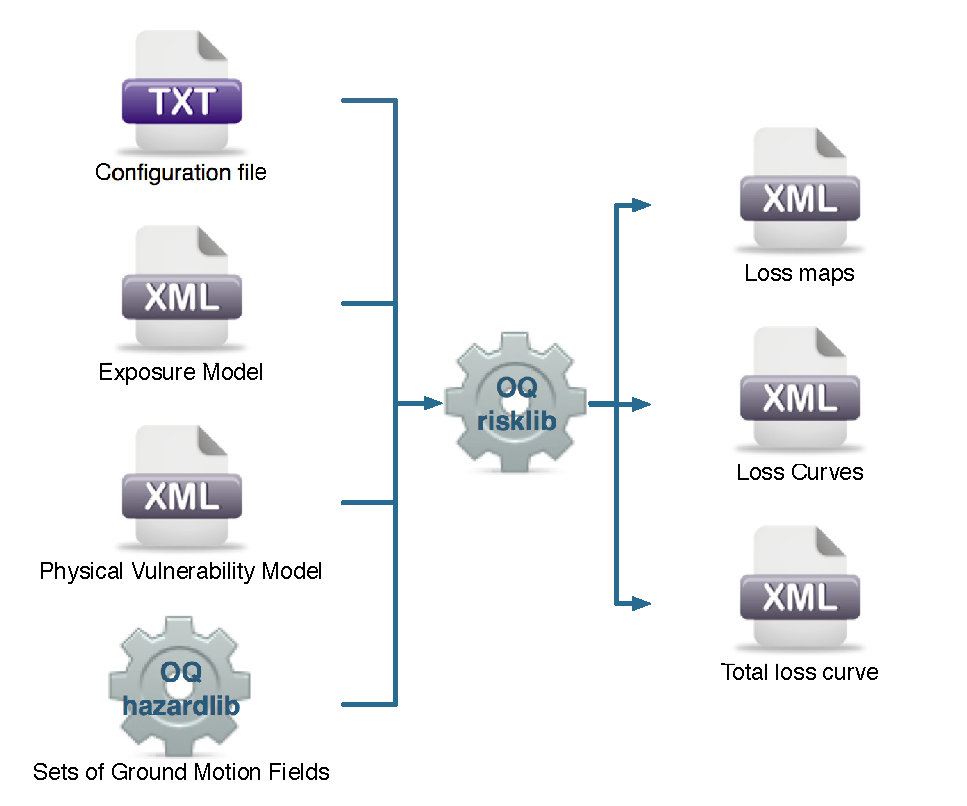
\includegraphics[width=9cm,height=7cm]{figures/risk/io-structure-event-based-risk.pdf}
\caption{Probabilistic Event-based Risk Calculator input/output structure.}
\label{fig:io-structure-event-based-risk}
\end{figure}


\section{Retrofit Benefit-Cost Ratio Analysis}
\index{OpenQuake-engine!Risk calculation workflows!Retrofit Benefit-Cost Ratio Analysis}
\label{sec:workflow_benefit_cost}
\input{oqum/risk/00_workflow_benefit_cost}

For further information regarding the theoretical background of the
methodologies used for each calculator, users are referred to the OpenQuake-
engine Book (Risk).

\cleardoublepage

   \cleardoublepage

\chapterimage{figures/chapter_head.pdf} % Chapter heading image
\chapter{Using the Hazard Module}
	\label{chap:hazinputs}
	This Chapter summarises the structure of the information necessary to define
a PSHA input model to be used with the \glsdesc{acr:oqe}.

Input data for probabilistic based seismic hazard analysis (Classical, Event
based, Disaggregation, and Uniform Hazard Spectra) are organised into:

\begin{itemize}

	\item A general configuration file.

    \item A file describing the Seismic Source System, that is the set of
	initial source models and associated epistemic uncertainties needed to
	model the seismic activity in the region of interest.

    \item A file describing the Ground Motion System, that is the set of
	ground motion prediction equations, per tectonic region type, needed to
	model the ground motion shaking in the region of interest.

\end{itemize}

Figure~\ref{fig:psha_input} summarises the structure of a PSHA input model
for the \glsdesc{acr:oqe} and the relationships between the different files.

\begin{figure}[!ht]
\centering
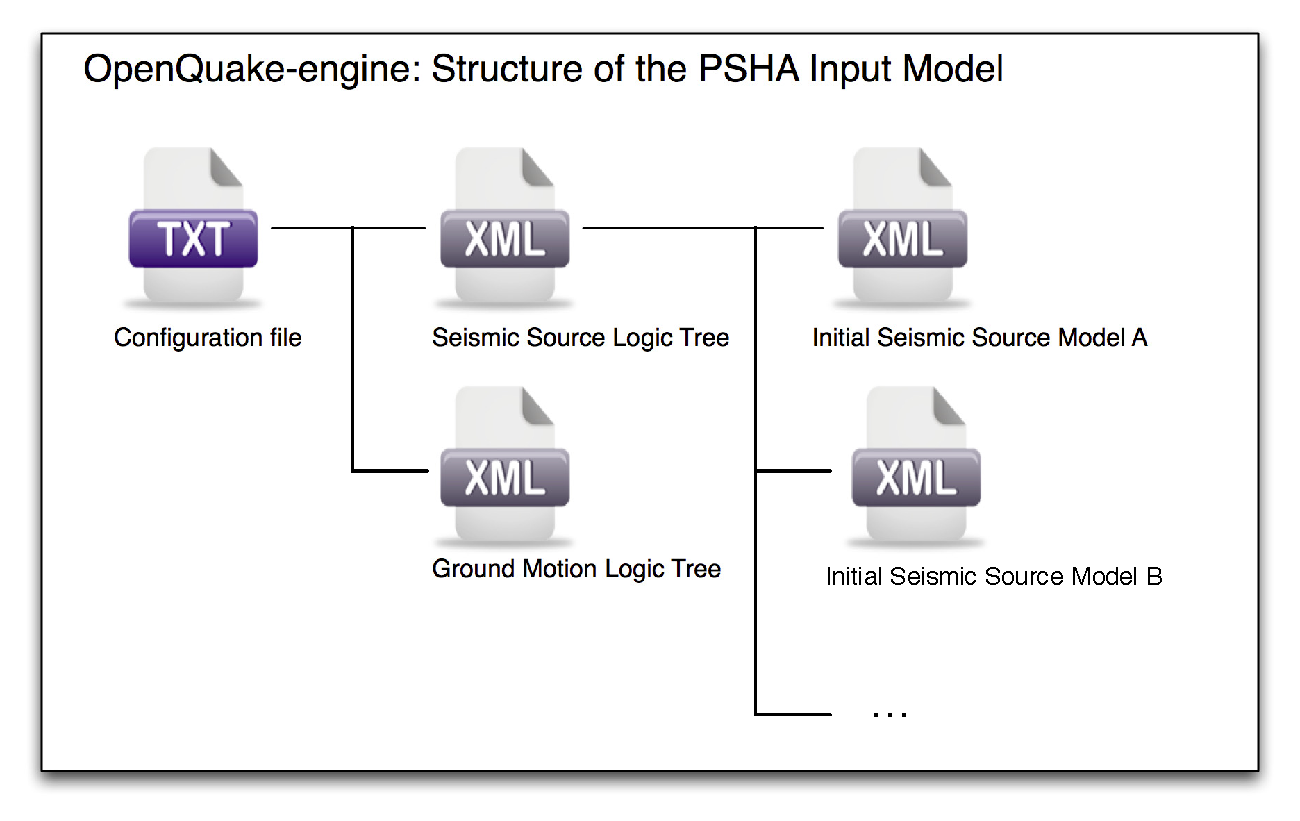
\includegraphics[width=14cm]{figures/hazard/psha_input_structure.pdf}
\caption{PSHA Input Model structure}
\label{fig:psha_input}
\end{figure}


\section{Defining Logic Trees}
The main components of a logic tree structure in the \glsdesc{acr:oqe} are the
following:

\begin{description}

    \item[branch]: the simplest component of a logic tree structure. A branch
	represent a possible interpretation of a value assignment for a specific type
	of uncertainty. It is fully described by the tuple (parameter or model,
	weight).

    \item[branching set]: it is a key component in the logic tree structure
	used by the \gls{acr:oqe}. It groups a set of branches i.e. alternative
	interpretations of a parameter or a model. Each branching set is defined by:

    \begin{itemize}

        \item An ID

        \item An uncertainty type (for a comprehensive list of the types of
		uncertainty currently supported see page~\pageref{list_epistemic_unc})

        \item One or more branches

    \end{itemize}

    This set of uncertainties can be applied to the whole initial  seismic
    source input model or just to a subset of seismic sources. The sum of the
    weights/probabilities assigned to the set  of branches always correspond
    to one.

    \item[branching level]: it is the largest container. It is not used in
	modelling uncertainty, but it is useful in maintaining a logic and an
	order in the structure of the tree.

\end{description}

Below we provide a simple schema illustrating the skeleton of xml file
containing the desciption of a logic tree:

\begin{minted}[firstline=1,firstnumber=1,fontsize=\footnotesize,frame=single,bgcolor=lightgray]{xml}
<logicTreeBranchingLevel branchingLevelID=ID>
    <logicTreeBranchSet branchSetID=ID
                        uncertaintyType=TYPE>
        <logicTreeBranch>
            <uncertaintyModel>VALUE</uncertaintyModel>
            <uncertaintyWeight>WEIGHT</uncertaintyWeight>
        </logicTreeBranch>
    </logicTreeBranchSet>
</logicTreeBranchingLevel>
\end{minted}

As it appears from this example, the structure of a logic tree is a set of
nested elements.

A schematic representation of the elemental components of a logic tree
structure is provided in Figure~\ref{glts}. A branching level identifies the
position where branching occurs while  a branch set identifies a collection of
branches (i.e. individual branches)  whose weights sum to 1.

\begin{figure}[!ht]
\centering
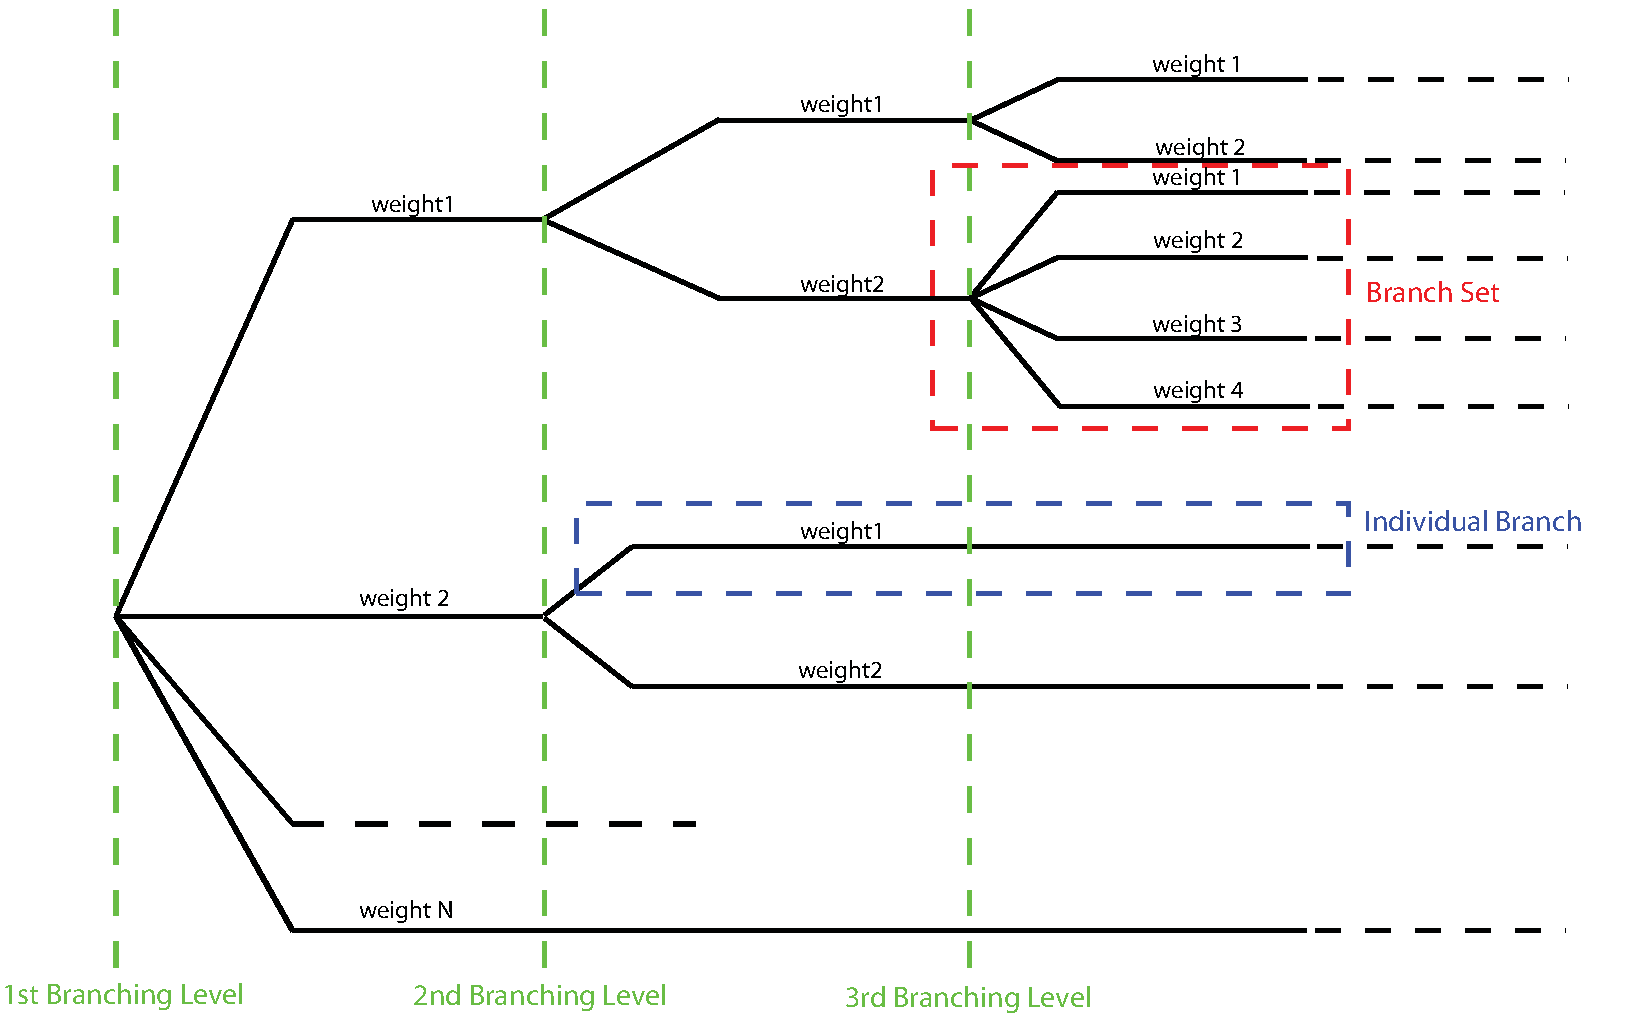
\includegraphics[width=13cm]{figures/hazard/GenericLogicTreeStructure.pdf}
\caption{Generic Logic Tree structure as described in terms of branching
levels, branch sets, and individual branches.}
\label{glts}
\end{figure}

\subsection{Logic trees as described in the nrml schema}

In the NRML schema, a logic tree structure is defined through the
\Verb+logicTree+ element:

\begin{minted}[firstline=1,firstnumber=1,fontsize=\footnotesize,frame=single,bgcolor=lightgray]{xml}
<logicTree logicTreeID="ID">
...
</logicTree>
\end{minted}

A \Verb+logicTree+ contains as a sequence of \Verb+logicTreeBranchingLevel+ elements. The position in the sequence of a \Verb+logicTreeBranchingLevel+ specifies the level of the tree where it is located. That is, the first \texttt{logicTreeBranchingLevel} element in the sequence represents  the first level in the tree, the second element the second level in the tree, and so on.

\begin{minted}[firstline=1,firstnumber=1,fontsize=\footnotesize,frame=single,bgcolor=lightgray]{xml}
<logicTree logicTreeID="ID">
	<logicTreeBranchingLevel branchingLevelID="ID_1">
		...
	</logicTreeBranchingLevel>
	<logicTreeBranchingLevel branchingLevelID="ID_2">
		...
	</logicTreeBranchingLevel>
	....
	<logicTreeBranchingLevel branchingLevelID="ID_N">
		...
	</logicTreeBranchingLevel>
</logicTree>
\end{minted}

There are no restrictions on the number of tree levels that can be defined.

A \Verb+logicTreeBranchingLevel+ is defined as a sequence of
\Verb+logicTreeBranchSet+ elements where each \Verb+logicTreeBranchSet+
defines a particular epistemic uncertainty inside a branching level.

A branch set has two required attributes: \Verb+branchSetID+ and
\Verb+uncertaintyType+. The latter defines the type of epistemic uncertainty this branch set is describing.

\begin{minted}[firstline=1,firstnumber=1,fontsize=\footnotesize,frame=single,bgcolor=lightgray]{xml}
<logicTree logicTreeID="ID">
...
	<logicTreeBranchingLevel branchingLevelID="ID_#">
		<logicTreeBranchSet branchSetID="ID_1"
			uncertaintyType="UNCERTAINTY_TYPE">
			...
		</logicTreeBranchSet>
		<logicTreeBranchSet branchSetID="ID_2"
			uncertaintyType="UNCERTAINTY_TYPE">
			...
		</logicTreeBranchSet>
		...
		<logicTreeBranchSet branchSetID="ID_N"
			uncertaintyType="UNCERTAINTY_TYPE">
			...
		</logicTreeBranchSet>
	</logicTreeBranchingLevel>
...
</logicTree>
\end{minted}

Possible values for the \Verb+uncertaintyType+ attribute are:

\label{list_epistemic_unc}
\begin{itemize}

    \item \Verb+gmpeModel+: indicates epistemic uncertainties on ground
	motion prediction equations

	\item \Verb+sourceModel+: indicates epistemic uncertainties on source models

    \item \Verb+maxMagGRRelative+: indicates relative (i.e. increments)
	epistemic uncertainties to be added (or subtracted, depending on the sign
	of the increment) to the Gutenberg-Richter maximum magnitude value.

    \item \Verb+bGRRelative+: indicates relative epistemic uncertainties
	to be applied to the Gutenberg-Richter b value.

    \item \Verb+abGRAbsolute+: indicates absolute (i.e. values used to replace
	original values) epistemic uncertainties on the Gutenberg-Richter a and b
	values.

    \item \Verb+maxMagGRAbsolute+: indicates (absolute) epistemic
	uncertainties on the Gutenberg-Richter maximum magnitude.
	
	\item \Verb+incrementalMFDAbsolute+: indicates (absolute) epistemic uncertainties on the incremental magnitude frequency distribution (i.e. alternative rates and/or minimum magnitude) of a specific source (can only be applied to individual sources)
	
	\item \Verb+simpleFaultGeometryAbsolute+: indicates alternative representations of the simple fault geometry for an individual simple fault source
	
	\item \Verb+simpleFaultDipRelative+: indicates a relative increase or decrease in fault dip for one or more simple fault sources
	
	\item \Verb+simpleFaultDipAbsolute+: indicates alternative values of fault dip for one or more simple fault sources
	
	\item \Verb+complexFaultGeometryAbsolute+: indicates alternative representations of complex fault geometry for an individual complex fault source

	\item \Verb+characteristicFaultGeometryAbsolute+: indicates alternative representations of the characteristic fault geometry for an individual characteristic fault source

\end{itemize}

There are no restrictions on the number of branch sets that can be defined inside a branching level.

A \Verb+branchSet+ is defined as a sequence of \Verb+logicTreeBranch+
elements, each specified by an \Verb+uncertaintyModel+ element (a string
identifying an uncertainty model; the content of the string varies with the \texttt{uncertaintyType} attribute value of the branchSet element) and the \texttt{uncertaintyWeight} element (specifying the probability/weight associated to the uncertaintyModel):

\begin{minted}[firstline=1,firstnumber=1,fontsize=\footnotesize,frame=single,bgcolor=lightgray]{xml}
< logicTree  logicTreeID="ID">
...
	< logicTreeBranchingLevel  branchingLevelID="ID_#">
		...
		< logicTreeBranchSet  branchSetID="ID_#"
				uncertaintyType="UNCERTAINTY_TYPE">
			< logicTreeBranch  branchID="ID_1">
				<uncertaintyModel>
				    UNCERTAINTY_MODEL
				</uncertaintyModel>
				<uncertaintyWeight>
				    UNCERTAINTY_WEIGHT
				</uncertaintyWeight>
			</ logicTreeBranch >
			...
			< logicTreeBranch  branchID="ID_N">
				<uncertaintyModel>
				    UNCERTAINTY_MODEL
				</uncertaintyModel>
				<uncertaintyWeight>
				    UNCERTAINTY_WEIGHT
				</uncertaintyWeight>
			</logicTreeBranch>
		</logicTreeBranchSet>
		...
	</logicTreeBranchingLevel>
...
</logicTree >
\end{minted}

Depending on the \Verb+uncertaintyType+ the content of the
\Verb+<uncertaintyModel>+ element changes:

\begin{itemize}

    \item if \Verb+uncertaintyType="gmpeModel"+, the uncertainty model
	contains the name of a ground motion prediction equation (a list of
	available GMPEs can be obtained using \texttt{oq info --gsims} and these
	are also documented at
	\href{http://docs.openquake.org/oq-hazardlib/0.24/openquake.hazardlib.gsim.html}{http://docs.openquake.org/oq-hazardlib/0.24/openquake.hazardlib.gsim.html}):

    \begin{minted}[firstline=1,firstnumber=1,fontsize=\footnotesize,frame=single,bgcolor=lightgray]{xml}
<uncertaintyModel>GMPE_NAME</uncertaintyModel>
	\end{minted}

    \item if \Verb+uncertaintyType="sourceModel"+, the uncertainty model
	contains the paths to a source model file, e.g.:

    \begin{minted}[firstline=1,firstnumber=1,fontsize=\footnotesize,frame=single,bgcolor=lightgray]{xml}
<uncertaintyModel>SOURCE_MODEL_FILE_PATH</uncertaintyModel>
	\end{minted}

    \item if \Verb+uncertaintyType="maxMagGRRelative"+, the uncertainty model
	contains the increment to be added (or subtracted, depending on the sign)
	to the Gutenberg-Richter maximum magnitude:

    \begin{minted}[firstline=1,firstnumber=1,fontsize=\footnotesize,frame=single,bgcolor=lightgray]{xml}
<uncertaintyModel>MAX_MAGNITUDE_INCREMENT</uncertaintyModel>
	\end{minted}

    \item if \Verb+uncertaintyType="bGRRelative"+, the uncertainty model
	contains the increment to be added (or subtracted, depending on the sign)
	to the Gutenberg-Richter b value:

    \begin{minted}[firstline=1,firstnumber=1,fontsize=\footnotesize,frame=single,bgcolor=lightgray]{xml}
<uncertaintyModel>B_VALUE_INCREMENT</uncertaintyModel>
	\end{minted}

    \item if \Verb+uncertaintyType="abGRAbsolute"+, the uncertainty model
	must contain one a and b pair:

    \begin{minted}[firstline=1,firstnumber=1,fontsize=\footnotesize,frame=single,bgcolor=lightgray]{xml}
<uncertaintyModel>A_VALUE B_VALUE</uncertaintyModel>
	\end{minted}

    \item if \Verb+uncertaintyType="maxMagGRAbsolute"+, the uncertainty
	model must contain one Gutenberg-Richter maximum magnitude value:

    \begin{minted}[firstline=1,firstnumber=1,fontsize=\footnotesize,frame=single,bgcolor=lightgray]{xml}
<uncertaintyModel>MAX_MAGNITUDE</uncertaintyModel>
	\end{minted}
	
	\item if \Verb+uncertaintyType="incrementalMFDAbsolute"+, the uncertainty model must contain an instance of the incremental MFD node:
	
    \begin{minted}[firstline=1,firstnumber=1,fontsize=\footnotesize,frame=single,bgcolor=lightgray]{xml}
<uncertaintyModel>
    <incrementalMFD
        minMag="MIN MAGNITUDE"
        binWidth="BIN WIDTH">
        <occurRates>RATE_1 RATE_2 ... RATE_N</occurRates>
    </incrementalMFD>
</uncertaintyModel>
    \end{minted}

    \item if \Verb+uncertaintyType="simpleFaultGeometryAbsolute"+ then the uncertainty model must contain a \emph{valid} instance of the \verb+simpleFaultGeometry+ node as described in section \ref{desc_simple_fault}

    \item if \Verb+uncertaintyType="simpleFaultDipRelative"+ then the uncertainty model must specify the number of degrees to increase (positive) or decrease (negative) the fault dip. Note that if this increase results in an adjusted fault dip greater than $90^{\circ}$ or less than $0^{\circ}$ an error will occur.
     
    \begin{minted}[firstline=1,firstnumber=1,fontsize=\footnotesize,frame=single,bgcolor=lightgray]{xml}
<uncertaintyModel>DIP_INCREMENT</uncertaintyModel>
	\end{minted}

	\item if \Verb+uncertaintyType="simpleFaultDipAbsolute"+ then the uncertainty model must specify the dip angle (in degrees)

    \begin{minted}[firstline=1,firstnumber=1,fontsize=\footnotesize,frame=single,bgcolor=lightgray]{xml}
<uncertaintyModel>DIP</uncertaintyModel>
	\end{minted}

    \item if \Verb+uncertaintyType="complexFaultGeometryAbsolute"+ then the uncertainty model must contain a \emph{valid} instance of the \verb+complexFaultGeometry+ source node as described in section \ref{desc_complex_fault}
    
    \item if \Verb+uncertaintyType="characteristicFaultGeometryAbsolute"+ then the uncertainty model must contain a \emph{valid} instance of the \verb+characteristicFaultGeometry+ source node, as described in section \ref{desc_characteristic_fault}
\end{itemize}

There are no restrictions on the number of \Verb+logicTreeBranch+ elements
that can be defined in a \Verb+logicTreeBranchSet+, as long as the uncertainty
weights sum to 1.0.

The \Verb+logicTreeBranchSet+ element offers also a number of optional
attributes allowing for complex tree definitions:

\begin{itemize}

    \item \Verb+applyToBranches+: specifies to which \Verb+logicTreeBranch+
	elements (one or more), in the previous branching level, the branch set
	is linked to. The linking is established by defining the IDs of the
	branches to link to:

	\begin{Verbatim}[commandchars=\\\{\}, samepage=true]
	applyToBranches="branchID1 branchID2 .... branchIDN"
	\end{Verbatim}

    The default is the keyword ALL, which means that a branch set is by
    default linked to all branches in the previous branching level. By
    specifying one or  more branches to which the branch set links to, non-
    symmetric logic trees can be defined.

    \item \Verb+applyToSources+: specifies to which source in a source model
	the uncertainty applies to. Sources are specified in terms of their IDs:

	\begin{Verbatim}[commandchars=\\\{\}, samepage=true]
	applyToSources="srcID1 srcID2 .... srcIDN"
	\end{Verbatim}

    \item \Verb+applyToSourceType+: specifies to which source type the
	uncertainty applies to.  Only one source typology can be defined
	(\Verb+area+, \Verb+point+, \Verb+simpleFault+, \Verb+complexFault+), e.g.:

	\begin{Verbatim}[commandchars=\\\{\}, samepage=true]
	applyToSources="area"
	\end{Verbatim}

    \item \Verb+applyToTectonicRegionType+: specifies to which tectonic
	region type the uncertainty applies to. Only one tectonic region type can
	be defined (\texttt{Active Shallow Crust}, \texttt{Stable
	Shallow Crust}, \texttt{Subduction Interface}, \texttt{Subduction}
	\texttt{IntraSlab}, \texttt{Volcanic}), e.g.:

	\begin{Verbatim}[commandchars=\\\{\}]
	applyToTectonicRegionType="Active Shallow Crust"
	\end{Verbatim}

\end{itemize}
\label{sec:hazard_logic_trees}

\section{The Seismic Source System}
The Seismic Source System contains the model (or the models) describing
position, geometry and activity of seismic sources of engineering importance
for a set of sites as well as the possible epistemic uncertainties to be
incorporated into the calculation of seismic hazard.



\subsection{The Seismic Source Logic Tree}

The structure of the Seismic Source Logic Tree consists of at least one
\gls{branchinglevel}. This branching level is the one used to define the
\gls{initialseismicsourceinputmodel} (or a number of initial seismic source
models, see Figure~\ref{fig:psha_input}).

The example provided below shows the simplest Seismic Source Logic Tree
structure that can be defined in a \gls{pshainputmodel} for \gls{acr:oqe}.
It's a logic tree with just one branching level containing one \gls{branchset}
with one branch used to define the initial seismic source model (its weight
will be equal to one).

\begin{minted}[firstline=1,firstnumber=1,fontsize=\footnotesize,frame=single,bgcolor=lightgray]{xml}
<?xml version="1.0" encoding="UTF-8"?>
<nrml xmlns:gml="http://www.opengis.net/gml"
      xmlns="http://openquake.org/xmlns/nrml/0.5">
    <logicTree logicTreeID="lt1">
        <logicTreeBranchingLevel branchingLevelID="bl1">
            <logicTreeBranchSet uncertaintyType="sourceModel"
                                branchSetID="bs1">
                <logicTreeBranch branchID="b1">
                    <uncertaintyModel>seismic_source_model.xml
                    </uncertaintyModel>
                    <uncertaintyWeight>1.0</uncertaintyWeight>
                </logicTreeBranch>
            </logicTreeBranchSet>
        </logicTreeBranchingLevel>
    </logicTree>
</nrml>
\end{minted}

The optional branching levels will contain rules that modify parameters of the
sources in the initial seismic source model.

For example, if the epistemic uncertainties to be considered are source
geometry and maximum magnitude, the modeller can create a logic tree structure
with three initial seismic source models (each one exploring a different
definition of the geometry of sources) and one branching level accounting for
the epistemic uncertainty on the maximum magnitude.

Below we provide an example of such logic tree structure. Note that the
uncertainty on the maximum magnitude is specified in terms of relative
increments with respect to the initial maximum magnitude defined for each
source in the initial seismic source models.

\inputminted[firstline=1,firstnumber=1,fontsize=\footnotesize,frame=single,linenos,bgcolor=lightgray]{xml}{oqum/hazard/verbatim/input_sslt_simple_lt.xml}
\captionof{listing}{Example source model logic tree structure\label{lst:example_source_model_logic_tree}}

Starting from \glsdesc{acr:oqe24}, it is also possible to split a source model
into several files and read them as if they were a single file. The file names
for the different files comprising a source model should be provided in the
source model logic tree file. For instance, a source model could be split by
tectonic region using the following syntax in the source model logic tree:

\begin{minted}[firstline=1,firstnumber=1,fontsize=\footnotesize,frame=single,bgcolor=lightgray]{xml}
<?xml version="1.0" encoding="UTF-8"?>
<nrml xmlns:gml="http://www.opengis.net/gml"
      xmlns="http://openquake.org/xmlns/nrml/0.5">
    <logicTree logicTreeID="lt1">
        <logicTreeBranchingLevel branchingLevelID="bl1">
            <logicTreeBranchSet uncertaintyType="sourceModel"
                                branchSetID="bs1">
                <logicTreeBranch branchID="b1">
                    <uncertaintyModel>
				     active_shallow_sources.xml
				     stable_shallow_sources.xml
				    </uncertaintyModel>
                    <uncertaintyWeight>1.0</uncertaintyWeight>
                </logicTreeBranch>
            </logicTreeBranchSet>
        </logicTreeBranchingLevel>
    </logicTree>
</nrml>
\end{minted}


\subsection{The Seismic Source Model}
\index{Input!Configuration file}

The structure of the xml file representing the seismic source model
corresponds to a list of sources, each one modelled using one out of the five
typologies currently supported. Below we provide a schematic example of a
seismic source model:

\begin{minted}[firstline=1,firstnumber=1,fontsize=\footnotesize,frame=single,bgcolor=lightgray]{xml}
< sourceModel  gml:id="ID">
	...
	< areaSource  gml:id="SOURCE_ID">
		<gml:name>SOURCE_NAME</gml:name>
		<tectonicRegion>TECT_REGION_TYPE</tectonicRegion>
		...
	</ areaSource >
	...
	< pointSource  gml:id="SOURCE_ID">
		<gml:name>SOURCE_NAME</gml:name>
		<tectonicRegion>TECT_REGION_TYPE</tectonicRegion>
		...
	</ pointSource >
	...
	< simpleFaultSource  gml:id="SOURCE_ID">
		<gml:name>SOURCE_NAME</gml:name>
		<tectonicRegion>TECT_REGION_TYPE</tectonicRegion>
		...
	</ simpleFaultSource >
	...
	< complexFaultSource  gml:id="SOURCE_ID">
		<gml:name>SOURCE_NAME</gml:name>
		<tectonicRegion>TECT_REGION_TYPE</tectonicRegion>
		...
	</ complexFaultSource >
	...
</ sourceModel >
\end{minted}


\label{sec:seismic_source_system}

\section{The Ground Motion System}
\index{Input!Ground motion system}
\label{sec:ground_motion_system}
The Ground Motion System defines the models and the possible epistemic
uncertainties related to ground motion modelling to be incorporated into the
calculation.

\subsection{The Ground Motion Logic Tree}
\index{Input!Ground motion logic tree}
\label{subsec:gmlt}

The structure of the \gls{groundmotionlogictree} consists of a list of ground
motion prediction equations for each tectonic region used to characterise the
sources in the PSHA input model.

The example below shows a simple \gls{groundmotionlogictree}. This logic tree
assumes that all the sources in the PSHA input model belong to ``Active
Shallow Crust'' and uses for calculation the \citet{chiou2008}
\gls{acr:gmpe}.

\begin{minted}[firstline=1,firstnumber=1,fontsize=\footnotesize,frame=single,bgcolor=lightgray]{xml}
<?xml version="1.0" encoding="UTF-8"?>
<nrml xmlns:gml="http://www.opengis.net/gml"
      xmlns="http://openquake.org/xmlns/nrml/0.5">
    <logicTree logicTreeID="lt1">
        <logicTreeBranchingLevel branchingLevelID="bl1">
            <logicTreeBranchSet uncertaintyType="gmpeModel"
                    branchSetID="bs1"
                    applyToTectonicRegionType="Active Shallow Crust">

                <logicTreeBranch branchID="b1">
                    <uncertaintyModel>
                    ChiouYoungs2008
                    </uncertaintyModel>
                    <uncertaintyWeight>1.0</uncertaintyWeight>
                </logicTreeBranch>

            </logicTreeBranchSet>
        </logicTreeBranchingLevel>
    </logicTree>
</nrml>
\end{minted}

\section{Configuration file}
\index{Input!Configuration file!Hazard}
\label{sec:hazard_configuration_file}
\input{oqum/hazard/01d_config.tex}
   \cleardoublepage

\chapterimage{figures/chapter_head.pdf} % Chapter heading image
\chapter{Hazard Calculations and Results}
	\label{chap:hazoutputs}
	\input{oqum/hazard/02_outputs}
   \cleardoublepage

\chapterimage{figures/chapter_head.pdf} % Chapter heading image
\chapter{Demonstrative Examples}
	\label{chap:hazdemos}
	\input{oqum/hazard/03_demos}
   \cleardoublepage

% ------------------------------------------------------ Part III: Risk Module -
\thispagestyle{empty}
\part{Risk}

\chapterimage{figures/chapter_head.pdf} % Chapter heading image
\chapter{Introduction to the Risk Module}
   \label{chap:riskintro}
	\index{OpenQuake-engine!Risk}

The seismic risk results are calculated using the \gls{acr:risklib}, 
an open-source suite of tools for seismic risk assessment and
loss estimation. This library is written in the Python programming language
and available in the form of a ``developers'' release at the following location:
\href{https://github.com/gem/oq-engine/tree/master/openquake/risklib}{https://github.com/gem/oq-engine/tree/master/openquake/risklib}.

The risk component of the \glsdesc{acr:oqe} can compute both scenario-based and
probabilistic seismic damage and risk using various approaches. The following
types of analysis are currently supported:

\begin{itemize}

    \item \textit{\textbf{Scenario Damage Assessment}}, for the
	calculation of damage distribution statistics for a portfolio of buildings
	from a single earthquake rupture scenario taking into account aleatory and
	epistemic ground-motion variability.

    \item \textit{\textbf{Scenario Risk Assessment}}, for the calculation of
	individual asset and portfolio loss statistics due to a single earthquake
	rupture scenario taking into account aleatory and epistemic ground-motion
	variability. Correlation in the vulnerability of different assets of the
	same typology can also be taken into consideration.

	\item \textit{\textbf{Classical Probabilistic Seismic Damage Analysis}}, for 
	the calculation of damage state probabilities over a specified time period,  
	and probabilistic collapse maps, starting from the hazard curves 
	computed following the classical integration procedure (\cite{cornell1968}, 
	\citet{mcguire1976}) as formulated by \cite{field2003}.

    \item \textit{\textbf{Classical Probabilistic Seismic Risk Analysis}}, for the
	calculation of loss curves and loss maps, starting from the hazard curves 
	computed following the classical integration procedure (\cite{cornell1968}, 
	\citet{mcguire1976}) as formulated by \cite{field2003}.

	\item \textit{\textbf{Stochastic Event Based Probabilistic Seismic Damage Analysis}}, 
	for the calculation of event damage tables starting from stochastic event sets.
	Other results such as damage-state-exceedance curves, probabilistic damage maps, 
	and average annual damages or collapses can be obtained by 
	post-processing the event damage tables.

	\item \textit{\textbf{Stochastic Event Based Probabilistic Seismic Risk Analysis}}, 
	for the calculation of event loss tables starting from stochastic event sets.
	Other results such as loss-exceedance curves, probabilistic loss maps, 
	and average annual losses can be obtained by 
	post-processing the event loss tables.

    \item \textit{\textbf{Retrofit Benefit-Cost Ratio Analysis}}, which is
	useful in estimating the net-present value of the potential benefits of
	performing retrofitting for a portfolio of assets (in terms of decreased
	losses in seismic events), measured relative to the upfront cost of
	retrofitting.

\end{itemize}

Each calculation workflow has a modular structure, so that intermediate
results can be saved and analyzed. Moreover, each calculator can be
extended independently of the others so that additional calculation options
and methodologies can be easily introduced, without affecting the overall
calculation workflow. Each workflow is described in more detail in the
following sections.

\section{Scenario Damage Assessment}
\index{OpenQuake-engine!Risk calculation workflows!Scenario Damage Assessment}
\label{sec:workflow_scenario_damage}
The scenario damage calculator computes damage distribution statistics for all
\glspl{asset} in a given \gls{exposuremodel} for a single specified
\gls{rupture}. Damage distribution statistics include the mean and standard
deviation of damage fractions for different damage states. This calculator
requires the definition of a finite \gls{rupturemodel}, an \gls{exposuremodel}
and a \gls{fragilitymodel}; the main results are the damage distribution
statistics per \gls{asset}, aggregated damage distribution statistics per
taxonomy, aggregated damage distribution statistics for the region, and
collapse maps, which contain the spatial distribution of the number or area of
collapsed buildings throughout the region of interest.

The \gls{rupture} characteristics---i.e. the magnitude, hypocenter and fault
geometry---are modelled as deterministic in the scenario calculators. Multiple
simulations of different possible \glspl{acr:gmf} due to the single
\gls{rupture} are generated, taking into consideration both the inter-event
variability of ground motions, and the intra-event residuals obtained from a
spatial correlation model for ground motion residuals. The use of logic trees
allows for the consideration of uncertainty in the choice of a ground motion
model for the given tectonic region.

As an alternative to computing the \glspl{acr:gmf} with \glsdesc{acr:oqe},
users can also provide their own sets of \glspl{acr:gmf} as input to the
scenario damage calculator.

\textbf{Note}: The damage simulation algorithm for the scenario damage 
calculator has changed starting from \glsdesc{acr:oqe39} to use a full
Monte Carlo simulation of damage states.

For each \gls{acr:gmf}, a damage state is simulated for each building for every
\gls{asset} in the \gls{exposuremodel} using the provided \gls{fragilitymodel},
and finally the mean damage distribution across all realizations is calculated.
The calculator also provides aggregated damage distribution statistics for the
portfolio, such as mean damage fractions for each taxonomy in the 
\gls{exposuremodel}, and the mean damage for the entire region of study.

The required input files required for running a scenario damage calculation
and the resulting output files are depicted in Figure~\ref{fig:io-structure-scenario-damage}.

\begin{figure}[ht]
\centering
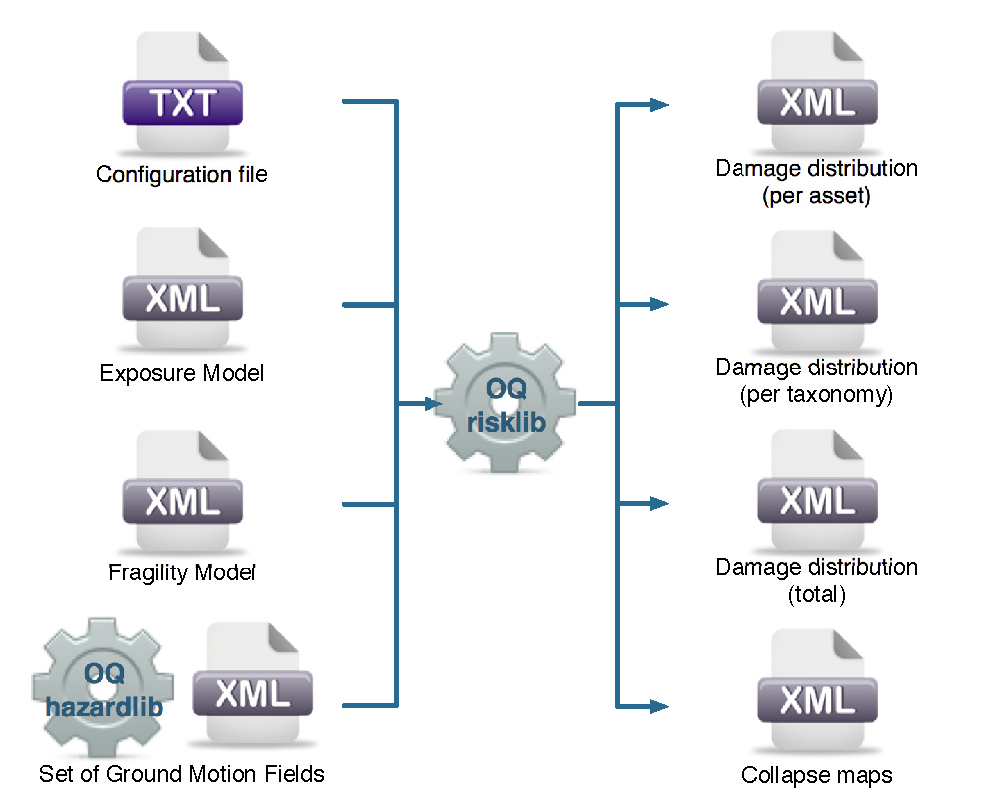
\includegraphics[width=9cm,height=7cm]{figures/risk/io-structure-scenario-damage.pdf}
\caption{Scenario Damage Calculator input/output structure.}
\label{fig:io-structure-scenario-damage}
\end{figure}

\gls{consequencemodel} files can also be
provided as inputs for a scenario damage calculation in addition to
\glspl{fragilitymodel} files, in order to estimate consequences based on the
calculated damage distribution. The user may provide one
\gls{consequencemodel} file corresponding to each loss type (amongst
structural, nonstructural, contents, and business interruption) for which a
\gls{fragilitymodel} file is provided. Whereas providing a
\gls{fragilitymodel} file for at least one loss type is mandatory for running
a Scenario Damage calculation, providing corresponding \gls{consequencemodel}
files is optional.


\section{Scenario Risk Assessment}
\index{OpenQuake-engine!Risk calculation workflows!Scenario Risk Assessment}
\label{sec:workflow_scenario_risk}
The scenario risk calculator computes loss statistics for all \glspl{asset} in
a given \gls{exposuremodel} for a single specified \gls{rupture}.
Loss statistics include the mean and standard deviation of ground-up losses
for each loss type considered in the analysis. Loss
statistics can currently be computed for five different loss types using this
calculator: structural losses, nonstructural losses, contents losses, downtime
losses, and occupant fatalities. This calculator requires the definition of a
finite \gls{rupturemodel}, an \gls{exposuremodel} and a
\gls{vulnerabilitymodel} for each loss type considered; the main results are
the loss statistics per \gls{asset} and mean loss maps.

The \gls{rupture} characteristics---i.e. the magnitude, hypocenter and fault
geometry---are modelled as deterministic in the scenario calculators. Multiple
simulations of different possible \glspl{acr:gmf} due to the single
\gls{rupture} are generated, taking into consideration both the inter-event
variability of ground motions, and the intra-event residuals obtained from a
spatial correlation model for ground motion residuals. The use of logic trees
allows for the consideration of uncertainty in the choice of a ground motion
model for the given tectonic region.

As an alternative to computing the \glspl{acr:gmf} with OpenQuake, users can
also provide their own sets of \glspl{acr:gmf} as input to the scenario risk
calculator.

For each \gls{acr:gmf} simulation, a loss ratio is sampled for every asset in
the \gls{exposuremodel} using the provided probabilistic
\gls{vulnerabilitymodel} taking into consideration the correlation model for
vulnerability of different \glspl{asset} of a given taxonomy. Finally loss
statistics, i.e., the mean loss and standard deviation of loss for
ground-up losses across all simulations, are calculated
for each \gls{asset}. Mean loss maps are also generated by this calculator,
describing the mean ground-up losses caused by the
scenario event for the different assets in the \gls{exposuremodel}.

The required input files required for running a scenario risk calculation and
the resulting output files are depicted in Figure~\ref{fig:io-structure-scenario-risk}.

\begin{figure}[ht]
\centering
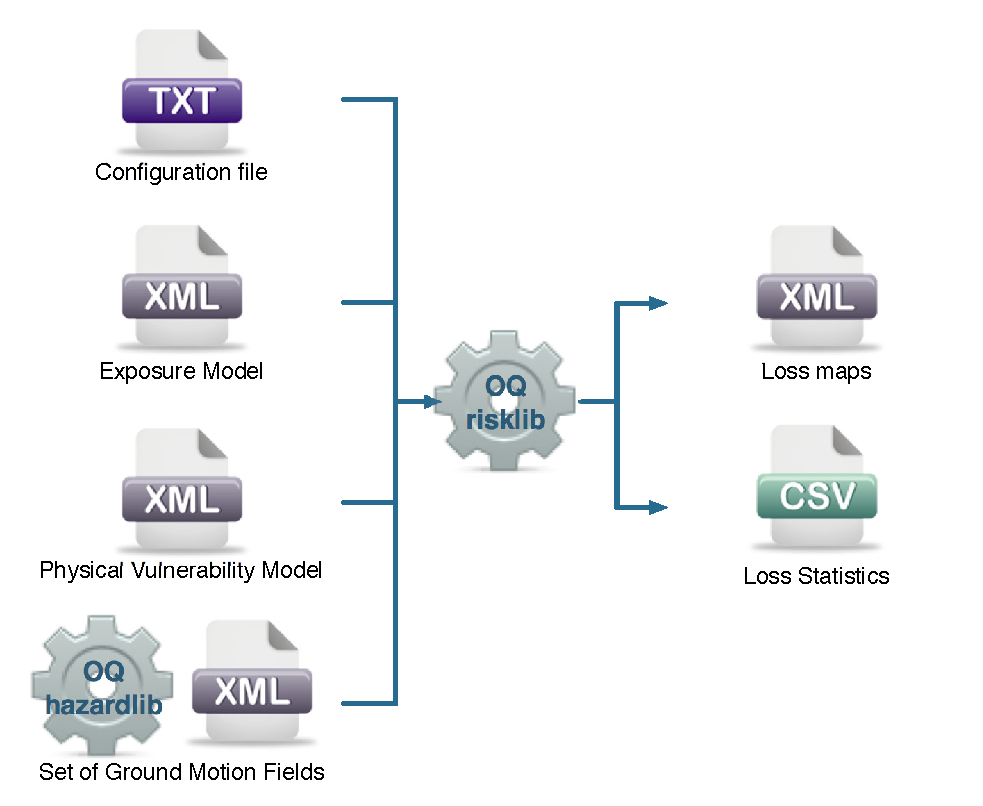
\includegraphics[width=9cm,height=7cm]{figures/risk/io-structure-scenario-risk.pdf}
\caption{Scenario Risk Calculator input/output structure.}
\label{fig:io-structure-scenario-risk}
\end{figure}


\section{Classical Probabilistic Seismic Damage Analysis}
\index{OpenQuake-engine!Risk calculation workflows!Classical Probabilistic Seismic Damage Analysis}
\label{sec:workflow_classical_damage}
\input{oqum/risk/00_workflow_classical_damage}

\section{Classical Probabilistic Seismic Risk Analysis}
\index{OpenQuake-engine!Risk calculation workflows!Classical Probabilistic Seismic Risk Analysis}
\label{sec:workflow_classical_risk}
\input{oqum/risk/00_workflow_classical_risk}

\section{Stochastic Event Based Probabilistic Seismic Damage Analysis}
\index{OpenQuake-engine!Risk calculation workflows!Event-Based Probabilistic Seismic Damage Analysis}
\label{sec:workflow_event_based_damage}
This calculator employs an event-based Monte Carlo simulation approach to
probabilistic damage assessment in order to estimate the damage distribution for
individual \glspl{asset} and aggregated damage distribution for a spatially
distributed portfolio of \glspl{asset} within a specified time period. The
calculator requires the definition of an \gls{exposuremodel}, a
\gls{fragilitymodel} for each loss type of interest with
\glspl{fragilityfunction} for each damage state for every typology represented 
in the \gls{exposuremodel}, and a \glsdesc{acr:ses} representative of the 
seismicity of the region over the specified time period. Damage state curves 
and damage maps corresponding to specified return periods can also be 
obtained using this calculator.

As an alternative to computing the \glspl{acr:gmf} with \glsdesc{acr:oqe},
users can also provide their own sets of \glspl{acr:gmf} as input to the
event-based damage calculator.

The main results of this calculator are the event damage tables; these 
tables describe the total number of buildings in each damage state for the
portfolio of \glspl{asset} for each seismic event in the \gls{acr:ses}.

Asset-level event damage tables are generated by the calculator, but are
not exportable in csv format due to the large file sizes that may be
involved. Interested users can access the asset-level event damage tables
within the datastore for the completed calculation.

% Uncomment after the addition of damage curves output
% Damage exceedance curves for each \gls{asset}, which describe 
% the probability of exceedance of different damage levels over the 
% specified time period, and damage maps for the region, which describe the 
% level of damage (for a given damage state) that has a given
% probability of exceedance over the specified time period. Aggregate damage
% exceedance curves can also be produced using this calculator; these
% describe the probability of exceedance of different damage levels for all
% \glspl{asset} in the portfolio.

This calculator relies on the probabilistic event-based hazard calculator,
which simulates the seismicity of the chosen time period $T$ by producing a
\gls{acr:ses}. For each \gls{rupture} generated by a \gls{seismicsource}, the
number of occurrences in the given time span $T$ is simulated by sampling the
corresponding probability distribution as given by $P_{rup}(k | T)$. A
\gls{acr:ses} is therefore a \textit{sample} of the full population of
\glspl{rupture} as defined by a \glsdesc{acr:ssm}. Each \gls{rupture} is
present zero, one or more times, depending on its probability. Symbolically,
we can define a \gls{acr:ses} as:
\begin{align}
SES(T) = \left\{k \times rup,\;k\sim P_{rup}(k | T)\;\;\forall\;rup\;in\;Src\;\forall\;Src\;in\;SSM\right\}
\end{align}
where $k$, the number of occurrences, is a random sample of $P_{rup}(k | T)$,
and $k \times rup$ means that \gls{rupture} $rup$ is repeated $k$ times in the
\gls{acr:ses}.

For each \gls{rupture} or event in the \glspl{acr:ses}, a spatially correlated
\gls{acr:gmf} realisation is generated, taking into consideration both the
inter-event variability of ground motions, and the intra-event residuals
obtained from a spatial correlation model for ground motion residuals (if one 
is specified in the job file). The use of logic trees allows for the 
consideration of uncertainty in the choice of a \glsdesc{acr:ssm}, and in the 
choice of \glspl{groundmotionmodel} for the different tectonic regions.

For each \gls{acr:gmf} realization, a damage state is siumulated for each
building of every \gls{asset} in the \gls{exposuremodel} using the provided
\gls{fragilitymodel}. The asset-level event damage table is saved to the datastore.
Time-averaged damage distributions at the asset-level can be obtained from
the event damage table. Finally damage state exceedance curves can be computed.

The required input files required for running a probabilistic stochastic
event-based damage calculation and the resulting output files are depicted in
Figure~\ref{fig:io-structure-event-based-damage}

\begin{figure}[ht]
\centering
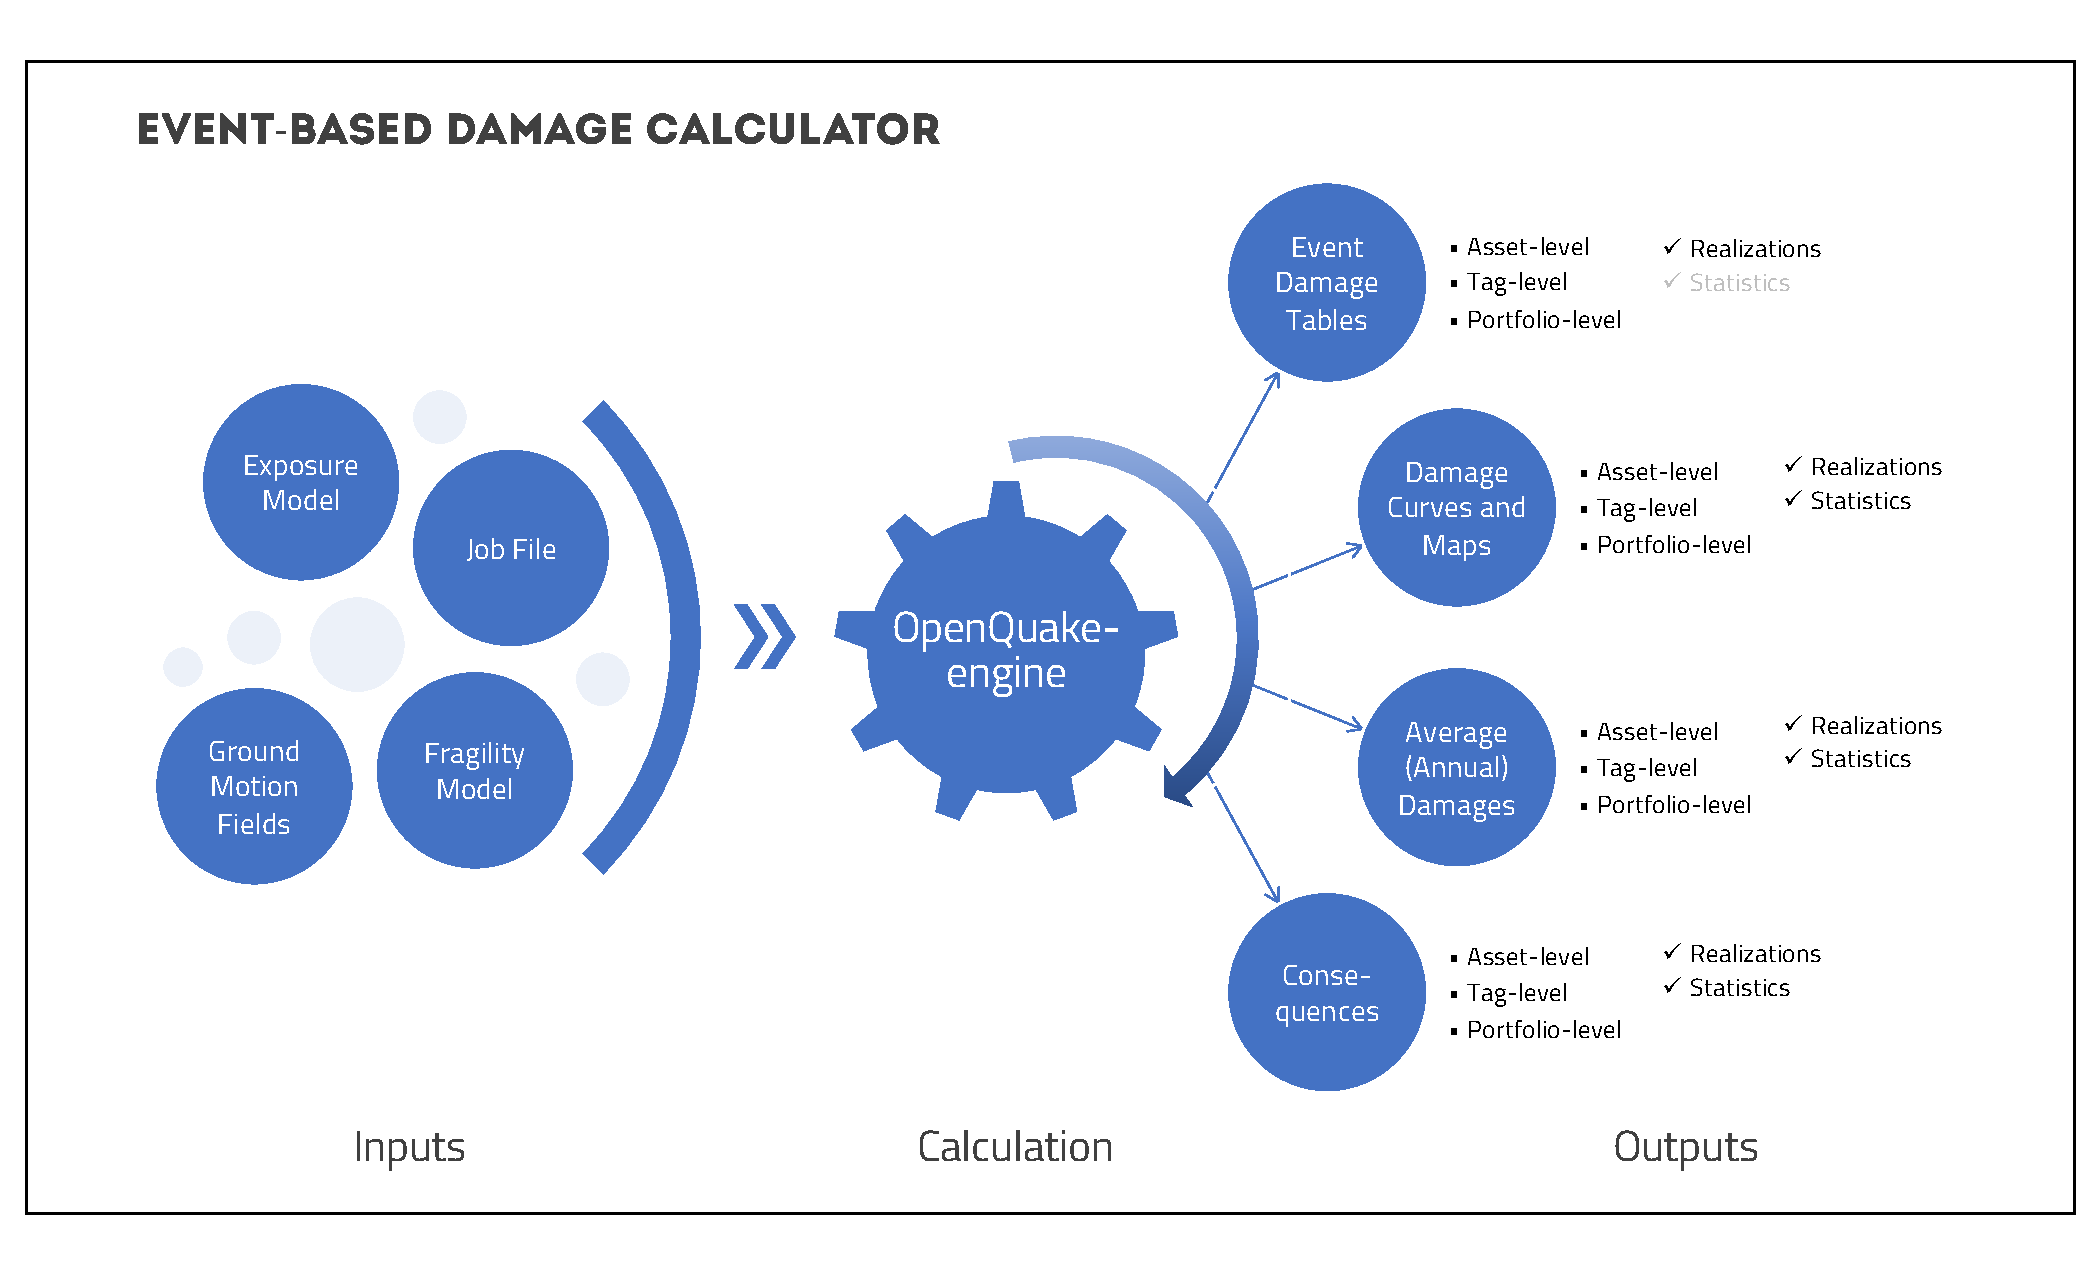
\includegraphics[width=12cm]{figures/risk/io-structure-event-based-damage.pdf}
\caption{Probabilistic Event-based Damage Calculator input/output structure.}
\label{fig:io-structure-event-based-damage}
\end{figure}

Similar to the scenario damage calculator, \gls{consequencemodel} files can also be
provided as inputs for an event-based damage calculation in addition to
\glspl{fragilitymodel} files, in order to estimate consequences based on the
calculated damage distribution. The user may provide one
\gls{consequencemodel} file corresponding to each loss type (amongst
structural, nonstructural, contents, and business interruption) for which a
\gls{fragilitymodel} file is provided. Whereas providing a
\gls{fragilitymodel} file for at least one loss type is mandatory for running
an Event-Based Damage calculation, providing corresponding \gls{consequencemodel}
files is optional.


\section{Stochastic Event Based Probabilistic Seismic Risk Analysis}
\index{OpenQuake-engine!Risk calculation workflows!Event-Based Probabilistic Seismic Risk Analysis}
\label{sec:workflow_event_based_risk}
This calculator employs an event-based Monte Carlo simulation approach to
probabilistic risk assessment in order to estimate the loss distribution for
individual \glspl{asset} and aggregated loss distribution for a spatially
distributed portfolio of \glspl{asset} within a specified time period. The
calculator requires the definition of an \gls{exposuremodel}, a
\gls{vulnerabilitymodel} for each loss type of interest with
\glspl{vulnerabilityfunction} for each taxonomy represented in the
\gls{exposuremodel}, and a \glsdesc{acr:ses} (also known as a
\textit{synthetic catalog}) representative of the seismicity of the region
over the specified time period. Loss curves and loss maps can currently be
calculated for five different loss types using this calculator: structural
losses, nonstructural losses, contents losses, downtime losses, and occupant
fatalities.

As an alternative to computing the \glspl{acr:gmf} with \glsdesc{acr:oqe},
users can also provide their own sets of \glspl{acr:gmf} as input to the
event-based risk calculator, starting from \gls{acr:oqe28}.

The main results of this calculator are loss
exceedance curves for each \gls{asset}, which describe the probability of
exceedance of different loss levels over the specified time period, and loss
maps for the region, which describe the loss values that have a given
probability of exceedance over the specified time period. Aggregate loss
exceedance curves can also be produced using this calculator; these
describe the probability of exceedance of different loss levels for all
\glspl{asset} in the portfolio. Finally, event loss tables can be produced
using this calculator; these tables describe the total loss across the
portfolio for each seismic event in the \gls{acr:ses}.

This calculator relies on the probabilistic event-based hazard calculator,
which simulates the seismicity of the chosen time period $T$ by producing a
\gls{acr:ses}. For each \gls{rupture} generated by a \gls{seismicsource}, the
number of occurrences in the given time span $T$ is simulated by sampling the
corresponding probability distribution as given by $P_{rup}(k | T)$. A
\gls{acr:ses} is therefore a \textit{sample} of the full population of
\glspl{rupture} as defined by a \glsdesc{acr:ssm}. Each \gls{rupture} is
present zero, one or more times, depending on its probability. Symbolically,
we can define a \gls{acr:ses} as:
\begin{align}
SES(T) = \left\{k \times rup,\;k\sim P_{rup}(k | T)\;\;\forall\;rup\;in\;Src\;\forall\;Src\;in\;SSM\right\}
\end{align}
where $k$, the number of occurrences, is a random sample of $P_{rup}(k | T)$,
and $k \times rup$ means that \gls{rupture} $rup$ is repeated $k$ times in the
\gls{acr:ses}.

For each \gls{rupture} or event in the \glspl{acr:ses}, a spatially correlated
\gls{acr:gmf} realisation is generated, taking into consideration both the
inter-event variability of ground motions, and the intra-event residuals
obtained from a spatial correlation model for ground motion residuals (if one 
is specified in the job file). The use of logic trees allows for the 
consideration of uncertainty in the choice of a \glsdesc{acr:ssm}, and in the 
choice of \glspl{groundmotionmodel} for the different tectonic regions.

For each \gls{acr:gmf} realization, a loss ratio is sampled for every
\gls{asset} in the \gls{exposuremodel} using the provided probabilistic
\gls{vulnerabilitymodel}, taking into consideration the correlation model for
vulnerability of different \glspl{asset} of a given taxonomy. Finally loss
exceedance curves are computed for ground-up losses.

The required input files required for running a probabilistic stochastic
event-based risk calculation and the resulting output files are depicted in
Figure~\ref{fig:io-structure-event-based-risk}

\begin{figure}[ht]
\centering
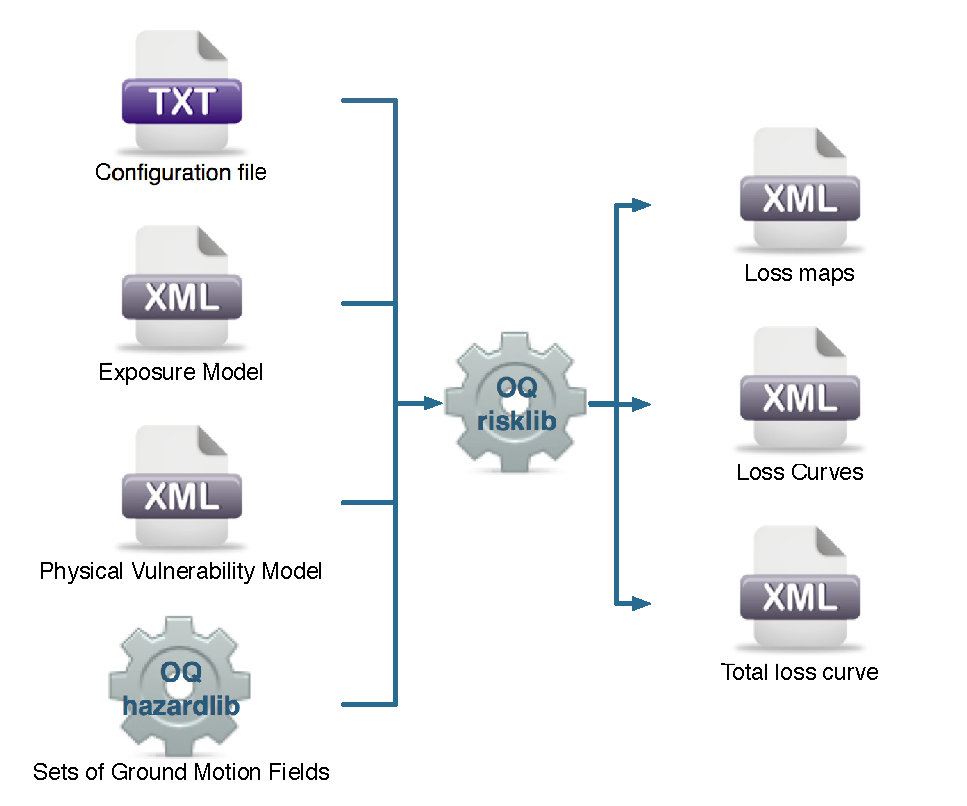
\includegraphics[width=9cm,height=7cm]{figures/risk/io-structure-event-based-risk.pdf}
\caption{Probabilistic Event-based Risk Calculator input/output structure.}
\label{fig:io-structure-event-based-risk}
\end{figure}


\section{Retrofit Benefit-Cost Ratio Analysis}
\index{OpenQuake-engine!Risk calculation workflows!Retrofit Benefit-Cost Ratio Analysis}
\label{sec:workflow_benefit_cost}
\input{oqum/risk/00_workflow_benefit_cost}

For further information regarding the theoretical background of the
methodologies used for each calculator, users are referred to the OpenQuake-
engine Book (Risk).

\cleardoublepage

   \cleardoublepage

\chapterimage{figures/chapter_head.pdf} % Chapter heading image
\chapter{Risk Input Models}
   \label{chap:riskinputs}
   \input{oqum/risk/01_inputs}
   \cleardoublepage

\chapterimage{figures/chapter_head.pdf} % Chapter heading image
\chapter{Using the Risk Module}
	\label{chap:riskcalculators}
	This Chapter summarises the structure of the information necessary to define
the different input data to be used with the \glsdesc{acr:oqe} risk
calculators. Input data for scenario-based and probabilistic seismic damage
and risk analysis using the \glsdesc{acr:oqe} are organised into:

\begin{itemize}

  \item An exposure model file in the NRML format, as described in 
    Section~\ref{sec:exposure}.

  \item A file describing the \gls{vulnerabilitymodel}
    (Section~\ref{sec:vulnerability}) for loss calculations, or a 
  	file describing the \gls{fragilitymodel} (Section~\ref{sec:fragility})
    for damage calculations. Optionally, a file describing the
    \gls{consequencemodel} (Section~\ref{sec:consequence}) can also be
  	provided in order to calculate losses from the estimated damage
  	distributions.

  \item A general calculation configuration file.

  \item Hazard inputs. These include hazard curves for the classical
    probabilistic damage and risk calculators, ground motion fields for the
    scenario damage and risk calculators, or stochastic event sets for the
    probabilistic event based calculators. As of \glsdesc{acr:oqe21}, in
    general, there are five different ways in which hazard calculation
    parameters or results can be provided to the \glsdesc{acr:oqe} in order to
    run the subsequent risk calculations:

    \begin{itemize}

      \item Use a single configuration file for running the hazard and risk
      calculations sequentially (preferred)

      \item Use separate configuration files for running the hazard and risk
      calculations sequentially (legacy)

      \item Use a configuration file for the risk calculation along with all
      hazard outputs from a previously completed, compatible
      \glsdesc{acr:oqe} hazard calculation

      % \item Use a configuration file for the risk calculation along with a
      % specific hazard output from a previously completed, compatible
      % \glsdesc{acr:oqe} hazard calculation

      \item Use a configuration file for the risk calculation along with
      hazard input files in the OpenQuake NRML format

    \end{itemize}

\end{itemize}

The file formats for \glspl{exposuremodel}, \glspl{fragilitymodel},
\glspl{consequencemodel}, and \glspl{vulnerabilitymodel} have been described
earlier in Chapter~\ref{chap:riskinputs}. The configuration file is the primary
file that provides the \glsdesc{acr:oqe} information regarding both the
definition of the input models (e.g. exposure, site parameters, fragility,
consequence, or vulnerability models) as well as the parameters governing the
risk calculation.

Information regarding the configuration file for running hazard calculations
using the \glsdesc{acr:oqe} can be found in
Section~\ref{sec:hazard_configuration_file}. Some initial mandatory parameters
of the configuration file common to all of the risk calculators are presented
in Listing~\ref{lst:config_example}. The remaining parameters that are
specific to each risk calculator are discussed in subsequent sections.

\begin{listing}[htbp]
  \inputminted[firstline=1,firstnumber=1,fontsize=\footnotesize,frame=single,linenos,bgcolor=lightgray]{ini}{oqum/risk/verbatim/config_example.ini}
  \caption{Example minimal risk calculation configuration file (\href{https://raw.githubusercontent.com/gem/oq-engine/master/doc/manual/oqum/risk/verbatim/config_example.xml}{Download example})}
  \label{lst:config_example}
\end{listing}

\begin{itemize}

  \item \Verb+description+: a parameter that can be used to include some
  information about the type of calculations that are going to be performed.

  \item \Verb+calculation_mode+: this parameter specifies the type of
  calculation to be run. Valid options for the \Verb+calculation_mode+ for
  the risk calculators are: \Verb+scenario_damage+, \Verb+scenario_risk+,
  \Verb+classical_damage+, \Verb+classical_risk+, \Verb+event_based_risk+,
  and \Verb+classical_bcr+.

  \item \Verb+exposure_file+: this parameter is used to specify the path to
  the \gls{exposuremodel} file. Typically this is the path to the xml file
  containing the exposure, or the xml file containing the metadata sections
  for the case where the assets are listed in one or more csv files. 
  For particularly large exposure models, it may be more convenient to provide 
  the path to a single compressed zip file that contains the exposure xml file
  and the exposure csv files (if any).

\end{itemize}

Depending on the type of risk calculation, other parameters besides the
aforementioned ones may need to be provided. We illustrate in the following
sections different examples of the configuration file for the different risk
calculators.


\section{Scenario Damage Calculator}
\label{sec:config_scenario_damage}
\input{oqum/risk/02_config_scenario_damage}

\section{Scenario Risk Calculator}
\label{sec:config_scenario_risk}
In order to run this calculator, the parameter \Verb+calculation_mode+ needs
to be set to \Verb+scenario_risk+. 

Most of the job configuration parameters required for running a scenario risk
calculation are the same as those described in the previous section for the
scenario damage calculator. The remaining parameters specific to the scenario
risk calculator are illustrated through the examples below.


\paragraph{Example 1}

This example illustrates a scenario risk calculation which uses a single
configuration file to first compute the ground motion fields for the given
rupture model and then calculate loss statistics for structural losses,
nonstructural losses, and insured structural losses, based on the ground
motion fields. The job configuration file required for running this scenario
risk calculation is shown in Listing~\ref{lst:config_scenario_risk_combined}.

\begin{listing}[htbp]
  \inputminted[firstline=1,firstnumber=1,fontsize=\footnotesize,frame=single,linenos,bgcolor=lightgray,label=job.ini]{ini}{oqum/risk/verbatim/config_scenario_risk_combined.ini}
  \caption{Example combined configuration file for a scenario risk calculation (\href{https://raw.githubusercontent.com/GEMScienceTools/oq-engine-docs/master/oqum/risk/verbatim/config_scenario_risk_combined.ini}{Download example})}
  \label{lst:config_scenario_risk_combined}
\end{listing}

Whereas a scenario damage calculation requires one or more fragility and/or
consequence models, a scenario risk calculation requires the user to specify
one or more vulnerability model files. Note that one or more of the following
parameters can be used in the same job configuration file to provide the
corresponding vulnerability model files:

\begin{itemize}

  \item \Verb+structural_vulnerability_file+: this parameter is used to
    specify the path to the structural \gls{vulnerabilitymodel} file

  \item \Verb+nonstructural_vulnerability_file+: this parameter is used to
    specify the path to the nonstructural\gls{vulnerabilitymodel} file

  \item \Verb+contents_vulnerability_file+: this parameter is used to
    specify the path to the contents \gls{vulnerabilitymodel} file

  \item \Verb+business_interruption_vulnerability_file+: this parameter is
    used to specify the path to the business interruption
    \gls{vulnerabilitymodel} file

  \item \Verb+occupants_vulnerability_file+: this parameter is used to
    specify the path to the occupants \gls{vulnerabilitymodel} file

\end{itemize}

It is important that the \Verb+lossCategory+ parameter in the metadata section
for each provided vulnerability model file (``structural'', ``nonstructural'',
``contents'', ``business\_interruption'', or ``occupants'') should match the
loss type defined in the configuration file by the relevant keyword above.

The remaining new parameters introduced in this example are the following:

\begin{itemize}

  \item \Verb+master_seed+: this parameter is used to control the random
    number generator in the loss ratio sampling process. If the same
    \Verb+master_seed+ is defined at each calculation run, the same random loss
    ratios will be generated, thus allowing reproducibility of the results.

  \item \Verb+asset_correlation+: if the uncertainty in the loss ratios
    has been defined within the \gls{vulnerabilitymodel}, users can specify
    a coefficient of correlation that will be used in the Monte Carlo sampling
    process of the loss ratios, between the assets that share the same
    \gls{taxonomy}. If the \Verb+asset_correlation+ is set to one,
    the loss ratio residuals will be perfectly correlated. On the other hand,
    if this parameter is set to zero, the loss ratios will be sampled
    independently. If this parameter is not defined, the
    \glsdesc{acr:oqe} will assume zero correlation in the vulnerability. As of
    \glsdesc{acr:oqe18}, \Verb+asset_correlation+ applies only to continuous
    \glspl{vulnerabilityfunction} using the lognormal or Beta distribution; 
    it does not apply to \glspl{vulnerabilityfunction} defined using the PMF
    distribution. Although partial correlation was supported in previous
    versions of the engine, beginning from \glsdesc{acr:oqe22}, values between
    zero and one are no longer supported due to performance considerations. The
    only two values permitted are \Verb+asset_correlation = 0+ and 
    \Verb+asset_correlation = 1+.

  \item \Verb+insured_losses+: this parameter specifies whether insured losses
    should be calculated; the default value of this parameter is \Verb+false+.
    In order for the \glsdesc{acr:oqe} to be able to compute insured losses, the
    insurance limits and deductibles must be listed for each asset in the 
    exposure model, as described in Example~5 in Section~\ref{sec:exposure}.

  \item \Verb+asset_loss_table+: this parameter
    specifies whether the individual asset and portfolio losses should be
    stored for each realization; the default value of this parameter is
    \Verb+false+ and only mean and standard deviation of the portfolio losses
    across all realizations are stored. If this flag is set to \Verb+true+, a
    matrix containing all of the losses is saved in the datastore and can be
    exported in the .npz format.

\end{itemize}

In this case, the ground motion fields will be computed at each of the
locations of the assets in the exposure model and for each of the intensity
measure types found in the provided set of vulnerability models. The above
calculation can be run using the command line:

\begin{minted}[fontsize=\footnotesize,frame=single,bgcolor=lightgray]{shell-session}
user@ubuntu:~\$ oq engine --run job.ini
\end{minted}

After the calculation is completed, a message similar to the following will be
displayed:

\begin{minted}[fontsize=\footnotesize,frame=single,bgcolor=lightgray]{shell-session}
Calculation 2735 completed in 10 seconds. Results:
  id | name
5328 | agglosses-rlzs
5329 | losses_by_asset
\end{minted}

All of the different ways of running a scenario damage calculation as
illustrated through the examples of the previous section are also applicable
to the scenario risk calculator, though the examples are not repeated here.


\section{Classical Probabilistic Seismic Damage Calculator}
\label{sec:config_classical_damage}
\input{oqum/risk/02_config_classical_damage}

\section{Classical Probabilistic Seismic Risk Calculator}
\label{sec:config_classical_risk}
In order to run this calculator, the parameter \Verb+calculation_mode+ needs
to be set to \Verb+classical_risk+.

Most of the job configuration parameters required for running a classical
probabilistic risk calculation are the same as those described in the previous
section for the classical probabilistic damage calculator. The remaining
parameters specific to the classical probabilistic risk calculator are
illustrated through the examples below.

\paragraph{Example 1}

This example illustrates a classical probabilistic risk calculation which uses
a single configuration file to first compute the hazard curves for the given
source model and ground motion model and then calculate loss exceedance curves
based on the hazard curves. An example job configuration file for running a
classical probabilistic risk calculation is shown in
Listing~\ref{lst:config_classical_risk_combined}.

\begin{listing}[htbp]
  \inputminted[firstline=1,firstnumber=1,fontsize=\footnotesize,frame=single,linenos,bgcolor=lightgray,label=job.ini]{ini}{oqum/risk/verbatim/config\_classical_risk\_combined.ini}
  \caption{Example combined configuration file for a classical probabilistic risk calculation (\href{https://raw.githubusercontent.com/gem/oq-engine/master/doc/manual/oqum/risk/verbatim/config\_classical\_risk\_combined.ini}{Download example})}
  \label{lst:config_classical_risk_combined}
\end{listing}

Apart from the calculation mode, the only difference with the example job
configuration file shown in Example~1 of
Section~\ref{sec:config_classical_damage} is the use of a vulnerability model
instead of a fragility model.

As with the Scenario Risk calculator, it is possible to specify one or more
\gls{vulnerabilitymodel} files in the same job configuration file, using the
parameters:

\begin{itemize}

  \item \Verb+structural_vulnerability_file+,

  \item \Verb+nonstructural_vulnerability_file+,

  \item \Verb+contents_vulnerability_file+,

  \item \Verb+business_interruption_vulnerability_file+, and/or

  \item \Verb+occupants_vulnerability_file+

\end{itemize}

It is important that the
\Verb+lossCategory+ parameter in the metadata section for each provided
vulnerability model file (``structural'', ``nonstructural'', ``contents'',
``business\_interruption'', or ``occupants'') should match the loss type
defined in the configuration file by the relevant keyword above.

In this case, the hazard curves will be computed at each of the locations of
the \glspl{asset} in the \gls{exposuremodel}, for each of the intensity
measure types found in the provided set of \glspl{vulnerabilitymodel}. The
above calculation can be run using the command line:

\begin{minted}[fontsize=\footnotesize,frame=single,bgcolor=lightgray]{shell-session}
user@ubuntu:~\$ oq engine --run job.ini
\end{minted}

After the calculation is completed, a message similar to the following will be
displayed:

\begin{minted}[fontsize=\footnotesize,frame=single,bgcolor=lightgray]{shell-session}
Calculation 2749 completed in 24 seconds. Results:
  id | name
3980 | Asset Loss Curves Statistics
3981 | Asset Loss Maps Statistics
3983 | Average Asset Loss Statistics
\end{minted}


\paragraph{Example 2}

This example illustrates a classical probabilistic risk calculation which uses
separate configuration files for the hazard and risk parts of a classical
probabilistic risk assessment. The first configuration file shown in
Listing~\ref{lst:config_classical_risk_hazard} contains input models and
parameters required for the computation of the hazard curves. The second
configuration file shown in Listing~\ref{lst:config_classical_risk} contains
input models and parameters required for the calculation of the loss
exceedance curves and probabilistic loss maps for a portfolio of \glspl{asset}
based on the hazard curves and \glspl{vulnerabilitymodel}.

\begin{listing}[htbp]
  \inputminted[firstline=1,firstnumber=1,fontsize=\footnotesize,frame=single,linenos,bgcolor=lightgray,label=job\_hazard.ini]{ini}{oqum/risk/verbatim/config\_classical\_hazard.ini}
  \caption{Example hazard configuration file for a classical probabilistic risk calculation (\href{https://raw.githubusercontent.com/gem/oq-engine/master/doc/manual/oqum/risk/verbatim/config\_classical\_hazard.ini}{Download example})}
  \label{lst:config_classical_risk_hazard}
\end{listing}

\begin{listing}[htbp]
  \inputminted[firstline=1,firstnumber=1,fontsize=\footnotesize,frame=single,linenos,bgcolor=lightgray,label=job\_risk.ini]{ini}{oqum/risk/verbatim/config\_classical\_risk.ini}
  \caption{Example risk configuration file for a classical probabilistic risk calculation (\href{https://raw.githubusercontent.com/gem/oq-engine/master/doc/manual/oqum/risk/verbatim/config\_classical\_risk.ini}{Download example})}
  \label{lst:config_classical_risk}
\end{listing}

Now, the above calculations described by the two configuration files
``job\_hazard.ini'' and ``job\_risk.ini'' can be run sequentially or
separately, as illustrated in Example~2 in
Section~\ref{sec:config_scenario_damage}. The new parameters introduced in the
above risk configuration file example
(Listing~\ref{lst:config_classical_risk}) are described below:

\begin{itemize}

	\item \Verb+lrem_steps_per_interval+: this parameter controls the number of
	  intermediate values between consecutive loss ratios (as defined in the 
	  \gls{vulnerabilitymodel}) that are considered in the risk calculations.
	  A larger number of loss ratios than those defined in each
	  \gls{vulnerabilityfunction} should be considered, in order to better
	  account for the uncertainty in the loss ratio distribution. If this
	  parameter is not defined in the configuration file, the \glsdesc{acr:oqe}
	  assumes the \Verb+lrem_steps_per_interval+ to be equal to 5. More details
	  are provided in the OpenQuake Book (Risk).

	\item \Verb+quantiles+: this parameter can be used to request
	  the computation of quantile loss curves for computations involving
	  non-trivial logic trees. The quantiles for which the loss curves should
	  be computed must be provided as a comma separated list. If this parameter
	  is not included in the configuration file, quantile loss curves will not
	  be computed. 

	\item \Verb+conditional_loss_poes+: this parameter can be used to request
	  the computation of probabilistic loss maps, which give the loss levels
	  exceeded at the specified probabilities of exceedance over the time
	  period specified by \Verb+risk_investigation_time+. The probabilities of
	  exceedance for which the loss maps should be computed must be provided as
	  a comma separated list. If this parameter is not included in the
	  configuration file, probabilistic loss maps will not be computed.

\end{itemize}


\section{Stochastic Event Based Seismic Damage Calculator}
\label{sec:config_event_based_damage}
The parameter \Verb+calculation_mode+ needs to be set to
\Verb+event_based_damage+ in order to use this calculator.

Most of the job configuration parameters required for running a stochastic
event based damage calculation are the same as those described in the previous
sections for the scenario damage calculator and the classical probabilistic damage
calculator. The remaining parameters specific to the stochastic event based
damage calculator are illustrated through the example below.


\paragraph{Example 1}

This example illustrates a stochastic event based damage calculation which uses
a single configuration file to first compute the \glspl{acr:ses} and
\glspl{acr:gmf} for the given source model and ground motion model, and then
calculate event loss tables, loss exceedance curves and probabilistic
loss maps for structural losses, nonstructural losses and occupants,
based on the \glspl{acr:gmf}. The job configuration file required for
running this stochastic event based damage calculation is shown in
Listing~\ref{lst:config_event_based_damage}.

\begin{listing}[htbp]
  \inputminted[firstline=1,firstnumber=1,fontsize=\scriptsize
  ,frame=single,bgcolor=lightgray,linenos,label=job.ini]{ini}{oqum/risk/verbatim/config_event_based_damage.ini}
  \caption{Example configuration file for running a stochastic event based damage calculation (\href{https://raw.githubusercontent.com/gem/oq-engine/master/doc/manual/oqum/risk/verbatim/config_event_based_damage.ini}{Download example})}
  \label{lst:config_event_based_damage}
\end{listing}

Similar to that the procedure described for the Scenario Damage calculator, a
Monte Carlo sampling process is also employed in this calculator to take into
account the uncertainty in the conditional loss ratio at a particular
intensity level. Hence, the parameters \Verb+asset_correlation+ and
\Verb+master_seed+ may be defined as previously described for the Scenario
Damage calculator in Section~\ref{sec:config_scenario_damage}. The parameter
``risk\_investigation\_time'' specifies the time period for which the average
damage values will be calculated, similar to the
Classical Probabilistic Damage calculator. If this parameter is not provided in
the risk job configuration file, the time period used is the same as that
specifed in the hazard calculation using the parameter ``investigation\_time''.

The new parameters introduced in this example are described below:

\begin{itemize}

  \item \Verb+minimum_intensity+: this optional parameter specifies the minimum
    intensity levels for each of the intensity measure types in the risk model.
    Ground motion fields where each ground motion value is less than the 
    specified minimum threshold are discarded. This helps speed up calculations
    and reduce memory consumption by considering only those ground motion fields
    that are likely to contribute to losses. It is also possible to set the same
    threshold value for all intensity measure types by simply providing a single
    value to this parameter. For instance: ``minimum\_intensity = 0.05'' would
    set the threshold to 0.05 g for all intensity measure types in the risk 
    calculation.
    If this parameter is not set, the \glsdesc{acr:oqe} extracts the minimum
    thresholds for each intensity measure type from the vulnerability
    models provided, picking the lowest intensity value for which a mean loss
    ratio is provided.

  \item \Verb+return_periods+: this parameter specifies the list of return
    periods (in years) for computing the asset / aggregate damage curves.
    If this parameter is not set, the \glsdesc{acr:oqe} uses a default set of
    return periods for computing the loss curves. The default return periods
    used are from the list: [5, 10, 25, 50, 100, 250, 500, 1000, ...], with 
    its upper bound limited by \Verb+(ses_per_logic_tree_path × investigation_time)+

    \begin{equation*}
    \begin{split}
    average\_damages & = sum(event\_damages) \\
                 & \div (hazard\_investigation\_time \times ses\_per\_logic\_tree\_path) \\
                 & \times risk\_investigation\_time
    \end{split}
    \end{equation*}

\end{itemize}

The above calculation can be run using the command line:

\begin{minted}[fontsize=\footnotesize,frame=single,bgcolor=lightgray]{shell-session}
user@ubuntu:~\$ oq engine --run job.ini
\end{minted}

Computation of the damage curves, and average damages for each
individual \gls{asset} in the \gls{exposuremodel} can be resource intensive,
and thus these outputs are not generated by default.

\section{Stochastic Event Based Seismic Risk Calculator}
\label{sec:config_event_based_risk}
The parameter \Verb+calculation_mode+ needs to be set to
\Verb+event_based_risk+ in order to use this calculator.

Most of the job configuration parameters required for running a stochastic
event based risk calculation are the same as those described in the previous
sections for the scenario risk calculator and the classical probabilistic risk
calculator. The remaining parameters specific to the stochastic event based
risk calculator are illustrated through the example below.


\paragraph{Example 1}

This example illustrates a stochastic event based risk calculation which uses
a single configuration file to first compute the \glspl{acr:ses} and
\glspl{acr:gmf} for the given source model and ground motion model, and then
calculate event loss tables, loss exceedance curves and probabilistic
loss maps for structural losses, nonstructural losses and occupants,
based on the \glspl{acr:gmf}. The job configuration file required for
running this stochastic event based risk calculation is shown in
Listing~\ref{lst:config_event_based_risk_combined}.

\begin{listing}[htbp]
  \inputminted[firstline=1,firstnumber=1,fontsize=\scriptsize
  ,frame=single,bgcolor=lightgray,linenos,label=job.ini]{ini}{oqum/risk/verbatim/config_event_based_risk_combined.ini}
  \caption{Example combined configuration file for running a stochastic event based risk calculation (\href{https://raw.githubusercontent.com/gem/oq-engine/master/doc/manual/oqum/risk/verbatim/config_event_based_risk_combined.ini}{Download example})}
  \label{lst:config_event_based_risk_combined}
\end{listing}

Similar to that the procedure described for the Scenario Risk calculator, a
Monte Carlo sampling process is also employed in this calculator to take into
account the uncertainty in the conditional loss ratio at a particular
intensity level. Hence, the parameters \Verb+asset_correlation+ and
\Verb+master_seed+ may be defined as previously described for the Scenario
Risk calculator in Section~\ref{sec:config_scenario_risk}. The parameter
``risk\_investigation\_time'' specifies the time period for which the event
loss tables and loss exceedance curves will be calculated, similar to the
Classical Probabilistic Risk calculator. If this parameter is not provided in
the risk job configuration file, the time period used is the same as that
specifed in the hazard calculation using the parameter ``investigation\_time''.

The new parameters introduced in this example are described below:

\begin{itemize}

  \item \Verb+minimum_intensity+: this optional parameter specifies the minimum
    intensity levels for each of the intensity measure types in the risk model.
    Ground motion fields where each ground motion value is less than the 
    specified minimum threshold are discarded. This helps speed up calculations
    and reduce memory consumption by considering only those ground motion fields
    that are likely to contribute to losses. It is also possible to set the same
    threshold value for all intensity measure types by simply providing a single
    value to this parameter. For instance: ``minimum\_intensity = 0.05'' would
    set the threshold to 0.05 g for all intensity measure types in the risk 
    calculation.
    If this parameter is not set, the \glsdesc{acr:oqe} extracts the minimum
    thresholds for each intensity measure type from the vulnerability
    models provided, picking the lowest intensity value for which a mean loss
    ratio is provided.

  \item \Verb+return_periods+: this parameter specifies the list of return
    periods (in years) for computing the aggregate loss curve.
    If this parameter is not set, the \glsdesc{acr:oqe} uses a default set of
    return periods for computing the loss curves. The default return periods
    used are from the list: [5, 10, 25, 50, 100, 250, 500, 1000, ...], with 
    its upper bound limited by \Verb+(ses_per_logic_tree_path × investigation_time)+

  \item \Verb+avg_losses+: this boolean parameter specifies whether the average
    asset losses over the time period ``risk\_investigation\_time'' should be
    computed. The default value of this parameter is \Verb+true+.

    \begin{equation*}
    \begin{split}
    average\_loss & = sum(event\_losses) \\
                 & \div (hazard\_investigation\_time \times ses\_per\_logic\_tree\_path) \\
                 & \times risk\_investigation\_time
    \end{split}
    \end{equation*}

\end{itemize}

The above calculation can be run using the command line:

\begin{minted}[fontsize=\footnotesize,frame=single,bgcolor=lightgray]{shell-session}
user@ubuntu:~\$ oq engine --run job.ini
\end{minted}

Computation of the loss tables, loss curves, and average losses for each
individual \gls{asset} in the \gls{exposuremodel} can be resource intensive,
and thus these outputs are not generated by default, unless instructed to by
using the parameters described above.


Users may also begin an event based risk calculation by providing a precomputed
set of \glspl{acr:gmf} to the \gls{acr:oqe}. The following example describes the
procedure for this approach.


\paragraph{Example 2}

This example illustrates a stochastic event based risk calculation which uses
a file listing a precomputed set of \glspl{acr:gmf}. These \glspl{acr:gmf} can
be computed using the \glsdesc{acr:oqe} or some other software. The
\glspl{acr:gmf} must be provided in either the \gls{acr:nrml} schema or the
csv format as presented in Section~\ref{subsec:output_event_based_psha}.
Listing~\ref{lst:output_gmf_xml} shows an example of a \glspl{acr:gmf} file in
the \gls{acr:nrml} schema and Table~\ref{output:gmf_event_based} shows an
example of a \glspl{acr:gmf} file in the csv format. If the \glspl{acr:gmf}
file is provided in the csv format, an additional csv file listing the site
ids must be provided using the parameter \Verb+sites_csv+. See
Table~\ref{output:sitemesh} for an example of the sites csv file, which
provides the association between the site ids in the \glspl{acr:gmf} csv file
with their latitude and longitude coordinates.

Starting from the input \glspl{acr:gmf}, the \gls{acr:oqe} can calculate event
loss tables, loss exceedance curves and probabilistic loss maps for structural
losses, nonstructural losses and occupants. The
job configuration file required for running this stochastic event based risk
calculation starting from a precomputed set of \glspl{acr:gmf} is shown in
Listing~\ref{lst:config_gmf_event_based_risk}.

\begin{listing}[htbp]
  \inputminted[firstline=1,firstnumber=1,fontsize=\scriptsize
  ,frame=single,bgcolor=lightgray,linenos,label=job.ini]{ini}{oqum/risk/verbatim/config_gmf_event_based_risk.ini}
  \caption{Example combined configuration file for running a stochastic event based risk calculation starting from a precomputed set of ground motion fields (\href{https://raw.githubusercontent.com/gem/oq-engine/master/doc/manual/oqum/risk/verbatim/config_gmf_event_based_risk.ini}{Download example})}
  \label{lst:config_gmf_event_based_risk}
\end{listing}


\paragraph{Additional parameters}

A few additional parameters related to the event based risk calculator that
may be useful for controlling specific aspects of the calculation are listed
below:

\begin{itemize}

  \item \Verb+individual_curves+: this boolean parameter is used to specify if
    the asset loss curves for each branch realization should be saved to the 
    datastore. For the asset loss curves output, by default the engine only 
    saves and exports statistical results, i.e. the mean and quantile asset 
    loss curves. If you want the asset loss curves for each of the individual 
    branch realizations, you must set \Verb+individual_curves=true+ in the job 
    file. Please take care: if you have hundreds of realizations, the data 
    transfer and disk space requirements will be orders of magnitude larger 
    than just returning the mean and quantile asset loss curves, and the 
    calculation might fail. The default value of \Verb+individual_curves+ is 
    \Verb+false+.

  \item \Verb+asset_correlation+: if the uncertainty in the loss ratios
    has been defined within the \gls{vulnerabilitymodel}, users can specify
    a coefficient of correlation that will be used in the Monte Carlo sampling
    process of the loss ratios, between the assets that share the same
    \gls{taxonomy}. If the \Verb+asset_correlation+ is set to one,
    the loss ratio residuals will be perfectly correlated. On the other hand,
    if this parameter is set to zero, the loss ratios will be sampled
    independently. If this parameter is not defined, the
    \glsdesc{acr:oqe} will assume zero correlation in the vulnerability. As of
    \glsdesc{acr:oqe18}, \Verb+asset_correlation+ applies only to continuous
    \glspl{vulnerabilityfunction} using the lognormal or Beta distribution; 
    it does not apply to \glspl{vulnerabilityfunction} defined using the PMF
    distribution. Although partial correlation was supported in previous
    versions of the engine, beginning from \glsdesc{acr:oqe22}, values between
    zero and one are no longer supported due to performance considerations. The
    only two values permitted are \Verb+asset_correlation = 0+ and 
    \Verb+asset_correlation = 1+.

  \item \Verb+ignore_covs+: this parameter controls the propagation of 
    vulnerability uncertainty to losses. The vulnerability functions using 
    continuous distributions (such as the lognormal distribution or beta 
    distribution) to characterize the uncertainty in the loss ratio 
    conditional on the shaking intensity level, specify the mean loss ratios 
    and the corresponding coefficients of variation for a set of intensity 
    levels. They are used to build the so called epsilon matrix within the 
    engine, which is how loss ratios are sampled from the distribution for 
    each asset. There is clearly a performance penalty associated with the 
    propagation of uncertainty in the vulnerability to losses. The epsilon 
    matrix has to be computed and stored, and then the worker processes have 
    to read it, which involves large quantities of data transfer and memory 
    usage. Setting \Verb+ignore_covs = true+ in the job file will result in 
    the engine using just the mean loss ratio conditioned on the shaking 
    intensity and ignoring the uncertainty. This tradeoff of not propagating 
    the vulnerabilty uncertainty to the loss estimates can lead to a 
    significant boost in performance and tractability. The default value of 
    \Verb+ignore_covs+ is \Verb+false+. 

\end{itemize}


\section{Retrofit Benefit-Cost Ratio Calculator}
\label{sec:config_benefit_cost}
\input{oqum/risk/02_config_benefit_cost}

\section{Exporting Risk Results}
\label{sec:risk_export}
To obtain a list of all risk calculations that have been previously run
(successfully or unsuccessfully), or that are currently running, the following
command can be employed:

\begin{minted}[fontsize=\footnotesize,frame=single,bgcolor=lightgray]{shell-session}
user@ubuntu:~\$ oq engine --list-risk-calculations
\end{minted}

or simply:

\begin{minted}[fontsize=\footnotesize,frame=single,bgcolor=lightgray]{shell-session}
user@ubuntu:~\$ oq engine --lrc
\end{minted}

Which will display a list of risk calculations as presented below.

\begin{minted}[fontsize=\footnotesize,frame=single,bgcolor=lightgray]{shell-session}
job_id |     status |          start_time |     description
     1 |   complete | 2015-12-02 08:50:30 | Scenario damage example
     2 |     failed | 2015-12-03 09:56:17 | Scenario risk example
     3 |   complete | 2015-12-04 10:45:32 | Scenario risk example
     4 |   complete | 2015-12-04 10:48:33 | Classical risk example
     5 |   complete | 2020-07-09 13:47:45 | Event based risk aggregation example     
\end{minted}

Then, in order to display a list of the risk outputs from a given job which has
completed successfully, the following command can be used:

\begin{minted}[fontsize=\footnotesize,frame=single,bgcolor=lightgray]{shell-session}
user@ubuntu:~\$ oq engine --list-outputs <risk_calculation_id>
\end{minted}

or simply:

\begin{minted}[fontsize=\footnotesize,frame=single,bgcolor=lightgray]{shell-session}
user@ubuntu:~\$ oq engine --lo <risk_calculation_id>
\end{minted}

which will display a list of outputs for the calculation requested, as
presented below:

\begin{minted}[fontsize=\footnotesize,frame=single,bgcolor=lightgray]{shell-session}
Calculation 5 results:
  id | name
  11 | Aggregate Event Losses
   1 | Aggregate Loss Curves
   2 | Aggregate Loss Curves Statistics
   3 | Aggregate Losses
   4 | Aggregate Losses Statistics
   5 | Average Asset Losses Statistics
  13 | Earthquake Ruptures
   6 | Events
   7 | Full Report
  10 | Input Files
  12 | Realizations
  14 | Source Loss Table
  15 | Total Loss Curves
  16 | Total Loss Curves Statistics
  17 | Total Losses
  18 | Total Losses Statistics
\end{minted}

Then, in order to export all of the risk calculation outputs in the
default file format (csv for most outputs), the following command can be used:

\begin{minted}[fontsize=\footnotesize,frame=single,bgcolor=lightgray]{shell-session}
user@ubuntu:~\$ oq engine --export-outputs <risk_calculation_id> <output_directory>
\end{minted}

or simply:

\begin{minted}[fontsize=\footnotesize,frame=single,bgcolor=lightgray]{shell-session}
user@ubuntu:~\$ oq engine --eos <risk_calculation_id> <output_directory>
\end{minted}

If, instead of exporting all of the outputs from a particular calculation,
only particular output files need to be exported, this can be achieved by
using the \Verb+--export-output+ option and providing the id of the required
output:

\begin{minted}[fontsize=\footnotesize,frame=single,bgcolor=lightgray]{shell-session}
user@ubuntu:~\$ oq engine --export-output <risk_output_id> <output_directory>
\end{minted}

or simply:

\begin{minted}[fontsize=\footnotesize,frame=single,bgcolor=lightgray]{shell-session}
user@ubuntu:~\$ oq engine --eo <risk_output_id> <output_directory>
\end{minted}


\cleardoublepage
   \cleardoublepage

\chapterimage{figures/chapter_head.pdf} % Chapter heading image
\chapter{Risk Results}
	\label{chap:riskoutputs}
	\input{oqum/risk/03_outputs}
   \cleardoublepage

\chapterimage{figures/chapter_head.pdf} % Chapter heading image
\chapter{Demonstrative Examples}
	\label{chap:riskdemos}
	The following sections describe the set of demos that have been compiled to
demonstrate some of the features and usage of the risk calculators of the
\glsdesc{acr:oqe}. These demos can be found in a public repository on GitHub at
the following link:
\href{https://github.com/gem/oq-engine/tree/master/demos/risk}
{https://github.com/gem/oq-engine/tree/master/demos/risk}.

These examples are purely demonstrative and are not intended to represent
accurately the seismicity, vulnerability or exposure characteristics of the
region selected, but simply to provide example input files that can be used
as a starting point for users planning to employ the \glsdesc{acr:oqe} in seismic
risk and loss estimation studies.

It is also noted that in the demonstrative examples presented in this section,
illustrations about the various messages from the engine displayed in the
command line interface are presented. These messages often contain information
about the calculation id and output id, which will certainly be different for
each user.

Following is the list of demos which illustrate how to use the \gls{acr:oqe} for
various scenario-based and probabilistic seismic damage and risk analyses:

\begin{itemize}

    \item ClassicalBCR
	\item ClassicalDamage
    \item ClassicalRisk
    \item EventBasedDamage
    \item EventBasedRisk
    \item ScenarioDamage
    \item ScenarioRisk

\end{itemize}

These seven demos use Nepal as the region of interest. An example
\gls{exposuremodel} has been developed for this region, comprising 9,063
assets distributed amongst 2,221 locations (due to the existence of more than
one \gls{asset} at the same location). A map with the distribution of the
number of buildings throughout Nepal is presented in Figure~\ref{fig:exposure-nepal}.

\begin{figure}[ht]
\centering
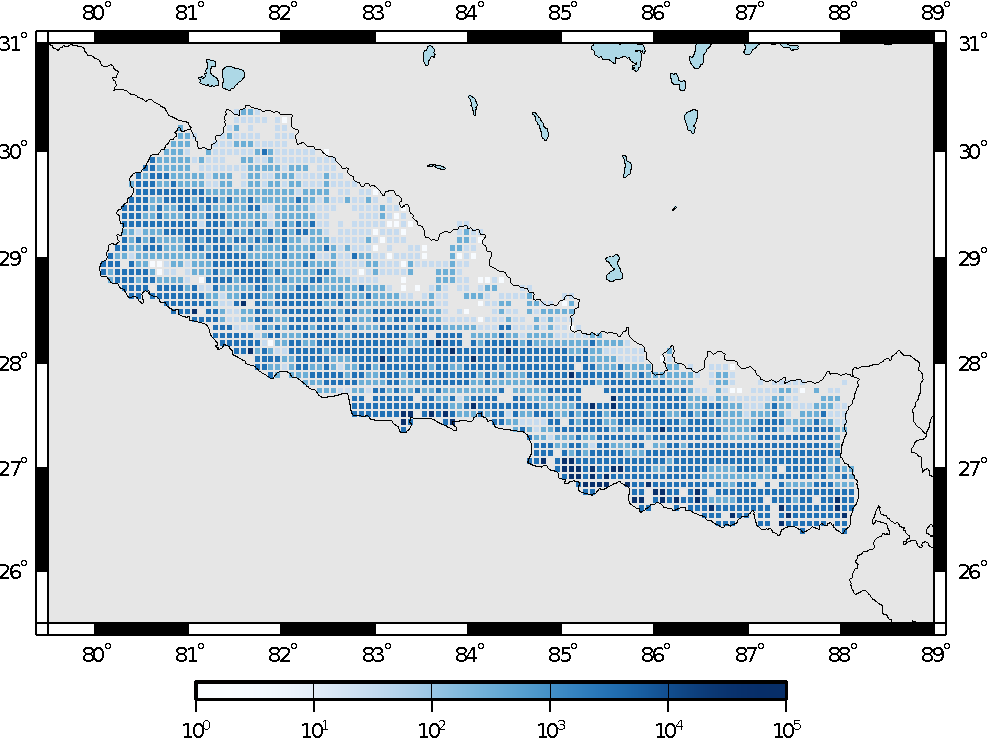
\includegraphics[width=12cm,height=8cm]{figures/risk/exposure-nepal.pdf}
\caption{Distribution of number of buildings in Nepal}
\label{fig:exposure-nepal}
\end{figure}

The building portfolio was organised into four classes for the rural areas
(adobe, dressed stone, unreinforced fired brick, wooden frames), and five
classes for the urban areas (the aforementioned typologies, in addition to
reinforced concrete buildings). For each one of these building typologies,
\glspl{vulnerabilityfunction} and \glspl{fragilityfunction} were collected
from the published literature available for the region. These input models are
only for demonstrative purposes and for further information about the building
characteristics of Nepal, users are advised to contact the National Society
for Earthquake Technology of Nepal (NSET -
\href{http://www.nset.org.np/}{http:www.nset.org.np/}).

The following sections include instructions not only on how to run the risk
calculations, but also on how to produce the necessary hazard inputs. Thus,
each demo comprises the configuration file, \gls{exposuremodel} and fragility or
vulnerability models fundamental for the risk calculations. Each demo folder
also a configuration file and the input models to produce the relevant hazard
inputs.


\section{Scenario Damage Demos}
\label{sec:demos_scenario_damage}
\input{oqum/risk/04_demos_scenario_damage}

\section{Scenario Risk Demos}
\label{sec:demos_scenario_risk}
\input{oqum/risk/04_demos_scenario_risk}

\section{Classical Probabilistic Seismic Damage Demos}
\label{sec:demos_classical_damage}
\input{oqum/risk/04_demos_classical_damage}

\section{Classical Probabilistic Seismic Risk Demos}
\label{sec:demos_classical_risk}
\input{oqum/risk/04_demos_classical_risk}

\section{Event Based Probabilistic Seismic Damage Demos}
\label{sec:demos_event_based_damage}
This demo uses the same probabilistic seismic hazard assessment (PSHA) model
described in the previous examples in Section~\ref{sec:demos_classical_damage}
and Section~\ref{sec:demos_classical_risk}. However, instead of hazard curves,
sets of ground motion fields will be generated by the hazard calculation of
this demo. Again, since there is only one branch in the logic tree, only one
set of ground motion fields will be used in the risk calculations. The hazard
and risk jobs are defined in a single configuration file for this demo. To
trigger the hazard and risk calculations the following command needs to be
used:

\begin{minted}[fontsize=\footnotesize,frame=single,bgcolor=lightgray]{shell-session}
user@ubuntu:~\$ oq engine --run job.ini
\end{minted}

and the following results are expected:

\begin{minted}[fontsize=\footnotesize,frame=single,bgcolor=lightgray]{shell-session}
Calculation 2 completed in 29 seconds. Results:
  id | name
  24 | Aggregate Event Damages
  30 | Aggregate Event Losses
  20 | Average Asset Damages
  21 | Average Asset Damages Statistics
  22 | Average Asset Losses
  23 | Average Asset Losses Statistics
  32 | Earthquake Ruptures
  25 | Events
  26 | Full Report
  27 | Ground Motion Fields
  28 | Hazard Curves
  29 | Input Files
  31 | Realizations
\end{minted}


\section{Event Based Probabilistic Seismic Risk Demos}
\label{sec:demos_event_based_risk}
\input{oqum/risk/04_demos_event_based_risk}

\section{Retrofit Benefit-Cost Ratio Demos}
\label{sec:demos_benefit_cost}
\input{oqum/risk/04_demos_benefit_cost}
   \cleardoublepage


%-------------------------------------------------------------------------------
%  BIBLIOGRAPHY
%-------------------------------------------------------------------------------

\chapter*{Bibliography}
\addcontentsline{toc}{chapter}{\textcolor{darkgray}{Bibliography}}
\section*{Books}
\printbibliography[heading=bibempty,type=book]
\section*{Articles}
\printbibliography[heading=bibempty,type=article]
\section*{Other Sources}
\printbibliography[heading=bibempty,nottype=book,nottype=article]
\cleardoublepage

%-------------------------------------------------------------------------------
%  INDEX & GLOSSARY
%-------------------------------------------------------------------------------

\printindex
\chapter*{Glossary}
\addcontentsline{toc}{chapter}{\textcolor{darkgray}{Glossary}}
\printglossary[type=acronym, title=List of Acronyms]
\printglossary[title=List of Terms]
\hfill \\ \thispagestyle{empty} \clearpage % ---------------- Final empty page -

\end{document}
